\documentclass[11pt,a4paper]{article}
% ============================================================
% Packages
% ============================================================
\usepackage[utf8]{inputenc}
\usepackage[T1]{fontenc}
\usepackage{lmodern}
\usepackage[english]{babel}
\usepackage{amsmath,amssymb,amsthm}
\usepackage{graphicx}
\usepackage{booktabs}
\usepackage[colorlinks=true, linkcolor=blue, citecolor=blue, urlcolor=blue, filecolor=blue]{hyperref}
\usepackage{cleveref}
\usepackage{algorithm}
\usepackage{algpseudocode}
\usepackage{tikz}
\usetikzlibrary{shapes.geometric, arrows.meta, positioning, fit, backgrounds}
\usepackage{xcolor}
\usepackage{listings}
\usepackage{subcaption}
\usepackage{multirow}
\usepackage{enumitem}
\usepackage{float}
\usepackage[margin=2.5cm]{geometry}
\usepackage{authblk}
\usepackage{natbib}
\bibliographystyle{plainnat}
% ============================================================
% Colors and Listings style
% ============================================================
\definecolor{codebg}{HTML}{F5F5F5}
\definecolor{codegreen}{HTML}{2E7D32}
\definecolor{codegray}{HTML}{757575}
\definecolor{codepurple}{HTML}{7B1FA2}
\definecolor{darkblue}{HTML}{1A237E}
\definecolor{darkred}{HTML}{B71C1C}
\definecolor{darkgreen}{HTML}{1B5E20}
\lstdefinestyle{pythonstyle}{
    backgroundcolor=\color{codebg},
    commentstyle=\color{codegreen},
    keywordstyle=\color{codepurple}\bfseries,
    stringstyle=\color{red!60!black},
    basicstyle=\ttfamily\footnotesize,
    breaklines=true,
    captionpos=b,
    keepspaces=true,
    numbers=left,
    numbersep=5pt,
    numberstyle=\tiny\color{codegray},
    showstringspaces=false,
    tabsize=2,
    frame=single,
    rulecolor=\color{gray!30},
    language=Python,
}
\lstset{style=pythonstyle}
% ============================================================
% TikZ styles
% ============================================================
\tikzstyle{agent} = [
    rectangle, rounded corners=4pt, minimum width=3.2cm, minimum height=1cm,
    text centered, draw=black!70, fill=blue!10, font=\small\bfseries
]
\tikzstyle{process} = [
    rectangle, rounded corners=2pt, minimum width=2.8cm, minimum height=0.85cm,
    text centered, draw=black!50, fill=orange!10, font=\small
]
\tikzstyle{decision} = [
    diamond, minimum width=2.8cm, minimum height=1.1cm,
    text centered, draw=black!60, fill=yellow!15, font=\small,
    aspect=2.8
]
\tikzstyle{data} = [
    rectangle, minimum width=2.2cm, minimum height=0.75cm,
    text centered, draw=black!40, fill=green!8, font=\small\itshape
]
\tikzstyle{verify} = [
    rectangle, rounded corners=2pt, minimum width=2.8cm, minimum height=0.85cm,
    text centered, draw=darkred!60, fill=red!5, font=\small
]
\tikzstyle{siv_style} = [
    rectangle, rounded corners=2pt, minimum width=2.8cm, minimum height=0.85cm,
    text centered, draw=darkgreen!70, fill=green!8, font=\small\bfseries
]
\tikzstyle{arrow} = [-{Stealth[length=2.5mm]}, thick]
\tikzstyle{arrowdashed} = [-{Stealth[length=2.5mm]}, dashed, gray]
% ============================================================
% algpseudocode try/catch (not natively supported)
% ============================================================
\algblock{Try}{EndTry}
\algblock{Catch}{EndCatch}
\algblockdefx[Try]{Try}{EndTry}[1][]{\textbf{try}}{\textbf{end try}}
\algblockdefx[Catch]{Catch}{EndCatch}[1][]{\textbf{catch} \textit{#1}}{\textbf{end catch}}
% ============================================================
% Title
% ============================================================
\title{%
    \textbf{Structured Hypothesis Testing for Multi-Agent\\
    Mathematical Reasoning in Large Language Models}
}
\author[1]{Marios Andreas Kalogerakis}
\author[1]{George Skiannis}
\affil[1]{Department of Computer Science, University of Ioannina, Ioannina, Greece}
\date{January, 2026}
% ============================================================
\begin{document}
% ============================================================
\maketitle
% ============================================================
\begin{abstract}
Large language models (LLMs) have demonstrated remarkable capabilities across diverse natural language tasks, yet mathematical reasoning remains a persistent challenge.
Single-pass inference frequently yields errors in multi-step arithmetic word problems due to hallucinated intermediate steps, misidentified operands, and sensitivity to irrelevant distractor information.
We introduce \textbf{MAS-SHT} (Multi-Agent Solver with Structured Hypothesis Testing), a framework that decomposes mathematical problem-solving into specialized agent roles: a \emph{Mathematician} (Architect) that produces a formal, self-verified JSON blueprint and a \emph{Programmer} (Engineer) that implements it as sandboxed executable Python code.
When the Programmer fails or produces an answer that disagrees with a zero-shot baseline, a confidence-gated \emph{Critic} agent performs structured peer review of the primary solution, generating a targeted correction and an independent rederivation.
If multiple candidates still disagree, an LLM-based \emph{Judge} resolves the conflict.
A rule-based process verification layer and a SymPy symbolic solver fallback provide additional robustness against code-generation failures at zero API cost.
We further introduce \textbf{Symbolic Inverse Verification (SIV)}, a deterministic, zero-API-call verification mechanism operating in two complementary layers.
\emph{Layer~1 (Execution Audit)} substitutes all numeric givens into the symbolic blueprint expression and compares the result to the Programmer's answer, detecting execution deviations without any LLM calls.
\emph{Layer~2 (Fault Localization)} algebraically inverts the forward equation chain using SymPy: for each given parameter, SIV treats it as unknown and solves backwards from the computed answer, identifying precisely which variable is inconsistent and enabling targeted Critic repair.
We note explicitly that SIV operates on the \emph{math$\to$math} layer: it verifies that the Programmer faithfully executed the Architect's blueprint, but cannot detect errors in the \emph{NL$\to$math} translation layer (i.e., a blueprint that models the problem incorrectly will still pass SIV if it is internally consistent).
This scope is complementary to---rather than competitive with---FOBAR \citep{jiang2024fobar}, which applies LLM-based backward reasoning that partially addresses the translation layer but is probabilistic and provides only a binary verdict; SIV provides deterministic, per-variable fault localization on the execution layer.
We evaluate MAS-SHT on five established benchmarks---GSM8K, GSM-Hard, GSM-Plus, GSM-Symbolic (P2), and SVAMP---under distractor-augmented conditions.
On a challenging mixed-benchmark set, MAS-SHT achieves 56.8\% accuracy with Qwen3-32B via Groq, compared to 5.4\% for the zero-shot baseline---a gain of \textbf{+51.4 percentage points}---while recording zero ``damage'' cases where a correct baseline answer was overwritten with an incorrect one.
A key finding is that when the Programmer successfully generates and executes code, it achieves 100\% accuracy; the entire performance gap is explained by blueprint construction failures.
On a standard GSM8K subset, the framework achieves 100\% accuracy compared to 90\% for the standalone baseline.
\end{abstract}
\noindent\textbf{Keywords:} Large Language Models, Mathematical Reasoning, Multi-Agent Systems, Hypothesis Testing, Chain-of-Thought, Code Generation, Process Verification, Symbolic Reasoning, Backward Verification
% ============================================================
\section{Introduction}
\label{sec:introduction}
% ============================================================
Mathematical word problem solving has long served as a benchmark for the reasoning capabilities of artificial intelligence systems.
Unlike factual retrieval or pattern matching, solving a multi-step arithmetic problem requires identifying relevant quantities, selecting appropriate operations, maintaining intermediate state, and arriving at a numerically precise answer.
Large language models (LLMs) such as GPT-4 \citep{openai2023gpt4}, LLaMA \citep{touvron2023llama}, and Gemini \citep{team2023gemini} have achieved impressive performance on benchmarks like GSM8K \citep{cobbe2021gsm8k}, yet error analysis reveals persistent failure modes: hallucinated operations, misidentified operands, fragility to surface-level rephrasing, and susceptibility to distractor information \citep{shi2023gsmsymbolic,li2024gsmplus}.
Two fundamental questions arise.
First, \emph{can decomposing the reasoning process into specialized agent roles reduce error rates compared to monolithic single-pass generation?}
Second, \emph{when the primary solution is uncertain, can structured exploration of alternative solution strategies recover the correct answer efficiently?}
These questions are particularly pressing on \emph{hard} benchmark variants: problems with larger numerical values, additional distractors, symbolic value substitutions, or structural variations that expose the brittleness of zero-shot reasoning.
Our experiments show that on such challenging benchmarks, zero-shot baseline accuracy can drop to near-zero (5.4\%), while the MAS-SHT framework recovers to 56.8\%---demonstrating that structured multi-agent reasoning is not merely incremental but can rescue problems that a powerful model completely fails on alone.
A further key finding clarifies \emph{where} the value lies: when the Programmer agent successfully generates and executes code, it achieves 100\% accuracy on our test set.
The entire performance gap between MAS-SHT and the baseline is therefore explained not by code execution failures, but by \emph{blueprint construction failures}---cases where the Mathematician cannot produce parseable JSON under token budget and complexity constraints.
This pinpoints blueprint construction as the single highest-leverage target for future improvement.
We present \textbf{MAS-SHT} (Multi-Agent Solver with Structured Hypothesis Testing), whose contributions are:
\begin{enumerate}[leftmargin=*,itemsep=3pt]
    \item \textbf{Architect--Engineer decomposition.} A \emph{Mathematician} agent produces a structured JSON blueprint containing identified unknowns, given values, ordered solution steps, Python-syntax equations, a self-verification estimate, and a distractor checklist. A \emph{Programmer} agent translates this blueprint into sandboxed executable Python code. If the Programmer fails after up to three repair attempts, a \emph{SymPy symbolic solver} re-evaluates the same equations with exact rational arithmetic.
    \item \textbf{Symbolic Inverse Verification (SIV).} After the Programmer produces an answer, SIV performs a two-layer deterministic audit at zero API cost.
    \emph{Layer~1 (Execution Audit)} evaluates the blueprint equations forward with all numeric givens substituted, producing a \texttt{blueprint\_answer}, and compares it to the Programmer's output---directly detecting any execution deviation.
    \emph{Layer~2 (Fault Localization)} inverts the symbolic equation chain: for each given variable, it solves backwards from the computed answer and checks whether the original value is recovered; \texttt{failed\_givens} names the inconsistent variables and the report is passed verbatim to the Critic for targeted repair.
    When the execution audit passes and all solvable givens reconstruct (confidence $\geq 0.90$), SHT is skipped entirely; when inconsistencies are detected, the specific localization report is forwarded to the Critic.
    \emph{Known scope limitation:} SIV operates on the \emph{math$\to$math} layer only. It verifies that the Programmer faithfully executed the Architect's blueprint equations, but cannot detect \emph{NL$\to$math} translation errors---i.e., a blueprint that models the problem incorrectly but is internally consistent will pass SIV's execution audit. This distinguishes SIV from FOBAR \citep{jiang2024fobar} (which applies LLM-based backward reasoning and partially addresses the translation layer, but is probabilistic and gives only a binary verdict): the two methods are \emph{orthogonal} and their combination is strictly stronger than either alone.
    \item \textbf{Self-verification in blueprint construction.} The Mathematician mentally traces through its own equations before finalizing the blueprint, storing the estimate in an \texttt{expected\_answer} field. This field is later consumed by the process verifier.
    \item \textbf{Rule-based process verification.} A zero-API-call verification pass cross-checks the generated code against the blueprint (givens consistency, equation variable coverage, answer sanity, expected-answer deviation). On failure, a second SymPy invocation is attempted.
    \item \textbf{Critic-based Structured Hypothesis Testing (SHT).} When the confidence gate detects uncertainty, a \emph{Critic} agent performs structured peer review: it diagnoses likely errors, generates a targeted correction (informed by the SIV fault localization report when available), and independently rederives a solution from scratch. This peer-review design avoids the correlated-error failure mode of naive parallel resampling.
    \item \textbf{Baseline as an active triage candidate.} The zero-shot baseline answer participates alongside the primary and critic-generated alternatives in majority-vote triage, providing an additional independent signal.
    \item \textbf{Distractor robustness evaluation.} A configurable hardening mechanism injects 1--3 irrelevant numerical sentences into problem statements, testing model resilience to distractors.
    \item \textbf{Comprehensive multi-benchmark evaluation} on five benchmarks (GSM8K, GSM-Hard, GSM-Plus, GSM-Symbolic P2, SVAMP) with two inference providers.
\end{enumerate}
\Cref{sec:related} surveys related work.
\Cref{sec:method} details the MAS-SHT architecture.
\Cref{sec:experiments} describes the experimental setup.
\Cref{sec:results} presents and analyzes results.
\Cref{sec:discussion} discusses implications and limitations.
\Cref{sec:conclusion} concludes.
% ============================================================
\section{Related Work}
\label{sec:related}
% ============================================================
\subsection{Chain-of-Thought and Step-by-Step Reasoning}
Chain-of-thought (CoT) prompting \citep{wei2022chain} demonstrated that eliciting intermediate reasoning steps substantially improves LLM performance on arithmetic tasks.
Subsequent work refined this through self-consistency decoding \citep{wang2023selfconsistency}, which samples multiple reasoning paths and selects the most common answer via majority voting.
Our confidence gate draws inspiration from self-consistency but operates across \emph{structurally distinct} solution strategies rather than temperature-varied samples of the same approach---a critical distinction that avoids correlated errors, as we discuss in \Cref{sec:discussion}.
\subsection{Program-Aided Language Models}
Program-aided language models (PAL) \citep{gao2023pal} and Program-of-Thought (PoT) \citep{chen2023program} offload computation to a Python interpreter, achieving higher accuracy by eliminating arithmetic errors in intermediate steps.
MAS-SHT adopts and extends this principle: the Programmer generates code constrained by a formal blueprint, reducing the likelihood of semantically incorrect programs.
When code generation fails, a SymPy-based algebraic solver provides arithmetic-guaranteed answers from the same blueprint equations---extending the PAL paradigm with a symbolic safety net.
\subsection{Multi-Agent Frameworks}
Multi-agent debate and collaboration frameworks have shown promise for improving LLM reasoning.
\citet{du2023improving} demonstrated that multi-agent debate among LLM instances improves factual accuracy.
\citet{liang2023encouraging} showed that assigning diverse roles enhances divergent thinking.
\citet{hong2023metagpt} introduced structured role assignment in coding agents, showing that explicit agent specialization reduces downstream errors.
Our Architect--Engineer pattern assigns complementary \emph{functional} roles: the Mathematician is responsible for mathematical formalization and the Programmer for faithful implementation, with their separation enforced at the prompt level.
\subsection{Verification and Self-Correction}
Verification-based approaches train or prompt models to check their own solutions.
\citet{lightman2023lets} introduced process reward models that evaluate each reasoning step.
\citet{weng2023large} explored self-verification through backward reasoning.
A closely related line of work is \textbf{FOBAR} \citep{jiang2024fobar}, which applies backward reasoning for answer verification: given the forward solution, the LLM is prompted to verify whether the original parameters can be recovered by working backwards.
MAS-SHT's Symbolic Inverse Verification (SIV) pursues the same \emph{cycle-consistency} idea but applies it to a different---and complementary---layer of the reasoning process.
FOBAR operates partially on the \emph{NL$\to$math} layer, using the LLM's natural-language reasoning to assess whether the problem was modelled correctly; SIV operates exclusively on the \emph{math$\to$math} layer, using a computer algebra system to verify that the Programmer faithfully executed the Architect's symbolic blueprint.
The two approaches are therefore \emph{orthogonal}: FOBAR is better positioned to catch translation errors (wrong problem model); SIV is better positioned to catch execution errors (correct model, wrong code) and provides per-variable fault localization rather than a binary verdict.
Their union is strictly stronger than either alone.
Within SIV's operating scope---the execution layer---three structural advantages arise over a hypothetical LLM-based execution verifier.
First, verification is \emph{deterministic}: given the same blueprint and answer, SIV always produces the same result; there is no LLM sampling noise.
Second, verification is \emph{free}: zero additional API calls are consumed.
Third, SIV is \emph{immune to correlated execution errors}: a model that consistently makes the same code-generation mistake will also make it during verification, whereas SymPy cannot.
Our rule-based process verification component is additionally related to \emph{peer review} frameworks in NLP \citep{gero2023selfeval}, but applied to mathematical derivation: the Critic is explicitly asked to identify the most likely error category before generating corrections.
\subsection{Symbolic and Hybrid Solvers}
Recent work has explored hybrid neural-symbolic approaches to improve numerical precision.
\citet{cobbe2021gsm8k} showed that verifier-guided search substantially improves accuracy on GSM8K.
ToRA \citep{gou2023tora} integrates tool augmentation with rationale generation, interleaving code calls with natural language reasoning steps.
Our SymPy fallback occupies a different point: rather than training a verifier or interleaving tool calls, we leverage a deterministic CAS to execute blueprint equations when code generation fails, providing exact arithmetic on correctly formulated equations.
SIV extends this CAS usage to the verification dimension, applying symbolic inversion as a post-hoc execution-fidelity audit.
\subsection{Rate-Limited Free-Tier LLM Evaluation}
Evaluating multi-agent LLM systems under practical inference constraints (free-tier APIs, token budgets, rate limits) is an underexplored engineering challenge.
MAS-SHT is specifically designed to operate within Groq's free tier of 100,000 tokens/day and 12 RPM for 32B-parameter models, using a realistic token estimation heuristic (input characters $\div$ 4 plus $0.35\times$ max output tokens) rather than pessimistic worst-case budgeting that would cause premature budget exhaustion.
\subsection{Mathematical Reasoning Benchmarks}
GSM8K \citep{cobbe2021gsm8k} remains the standard benchmark for grade-school math reasoning.
GSM-Hard \citep{gao2023pal} replaces numbers with larger values.
GSM-Plus \citep{li2024gsmplus} applies systematic perturbations covering digit expansion, distraction insertion, reversing operations, and numerical substitution.
GSM-Symbolic \citep{shi2023gsmsymbolic} introduces symbolic value variations at three complexity levels (main, P1, P2).
SVAMP \citep{patel2021svamp} tests cross-domain arithmetic reasoning with structural variation.
We evaluate on all five benchmarks.
% ============================================================
\section{Method}
\label{sec:method}
% ============================================================
\subsection{System Overview}
MAS-SHT processes each mathematical word problem through an eight-stage pipeline illustrated in \Cref{fig:architecture}:
(1)~zero-shot \emph{Baseline} generation,
(2)~\emph{Mathematician} blueprint construction with self-verification,
(3)~\emph{Programmer} code generation, sandboxed execution, and repair loop,
(3b)~\emph{Rule-based process verification} with optional SymPy fallback,
(3c)~\emph{Symbolic Inverse Verification (SIV)}: a two-layer audit comprising a forward execution check (Layer~1) and per-variable inverse fault localization (Layer~2), both using SymPy CAS at zero API cost,
(4)~\emph{Confidence Gate} evaluation (with SIV execution audit as the highest-priority criterion),
(5)~\emph{Critic-based Hypothesis Testing} with SIV-informed targeted correction and independent rederivation, and---if candidates disagree---
(6)~\emph{LLM Judge} arbitration.
\begin{figure}[t]
\centering
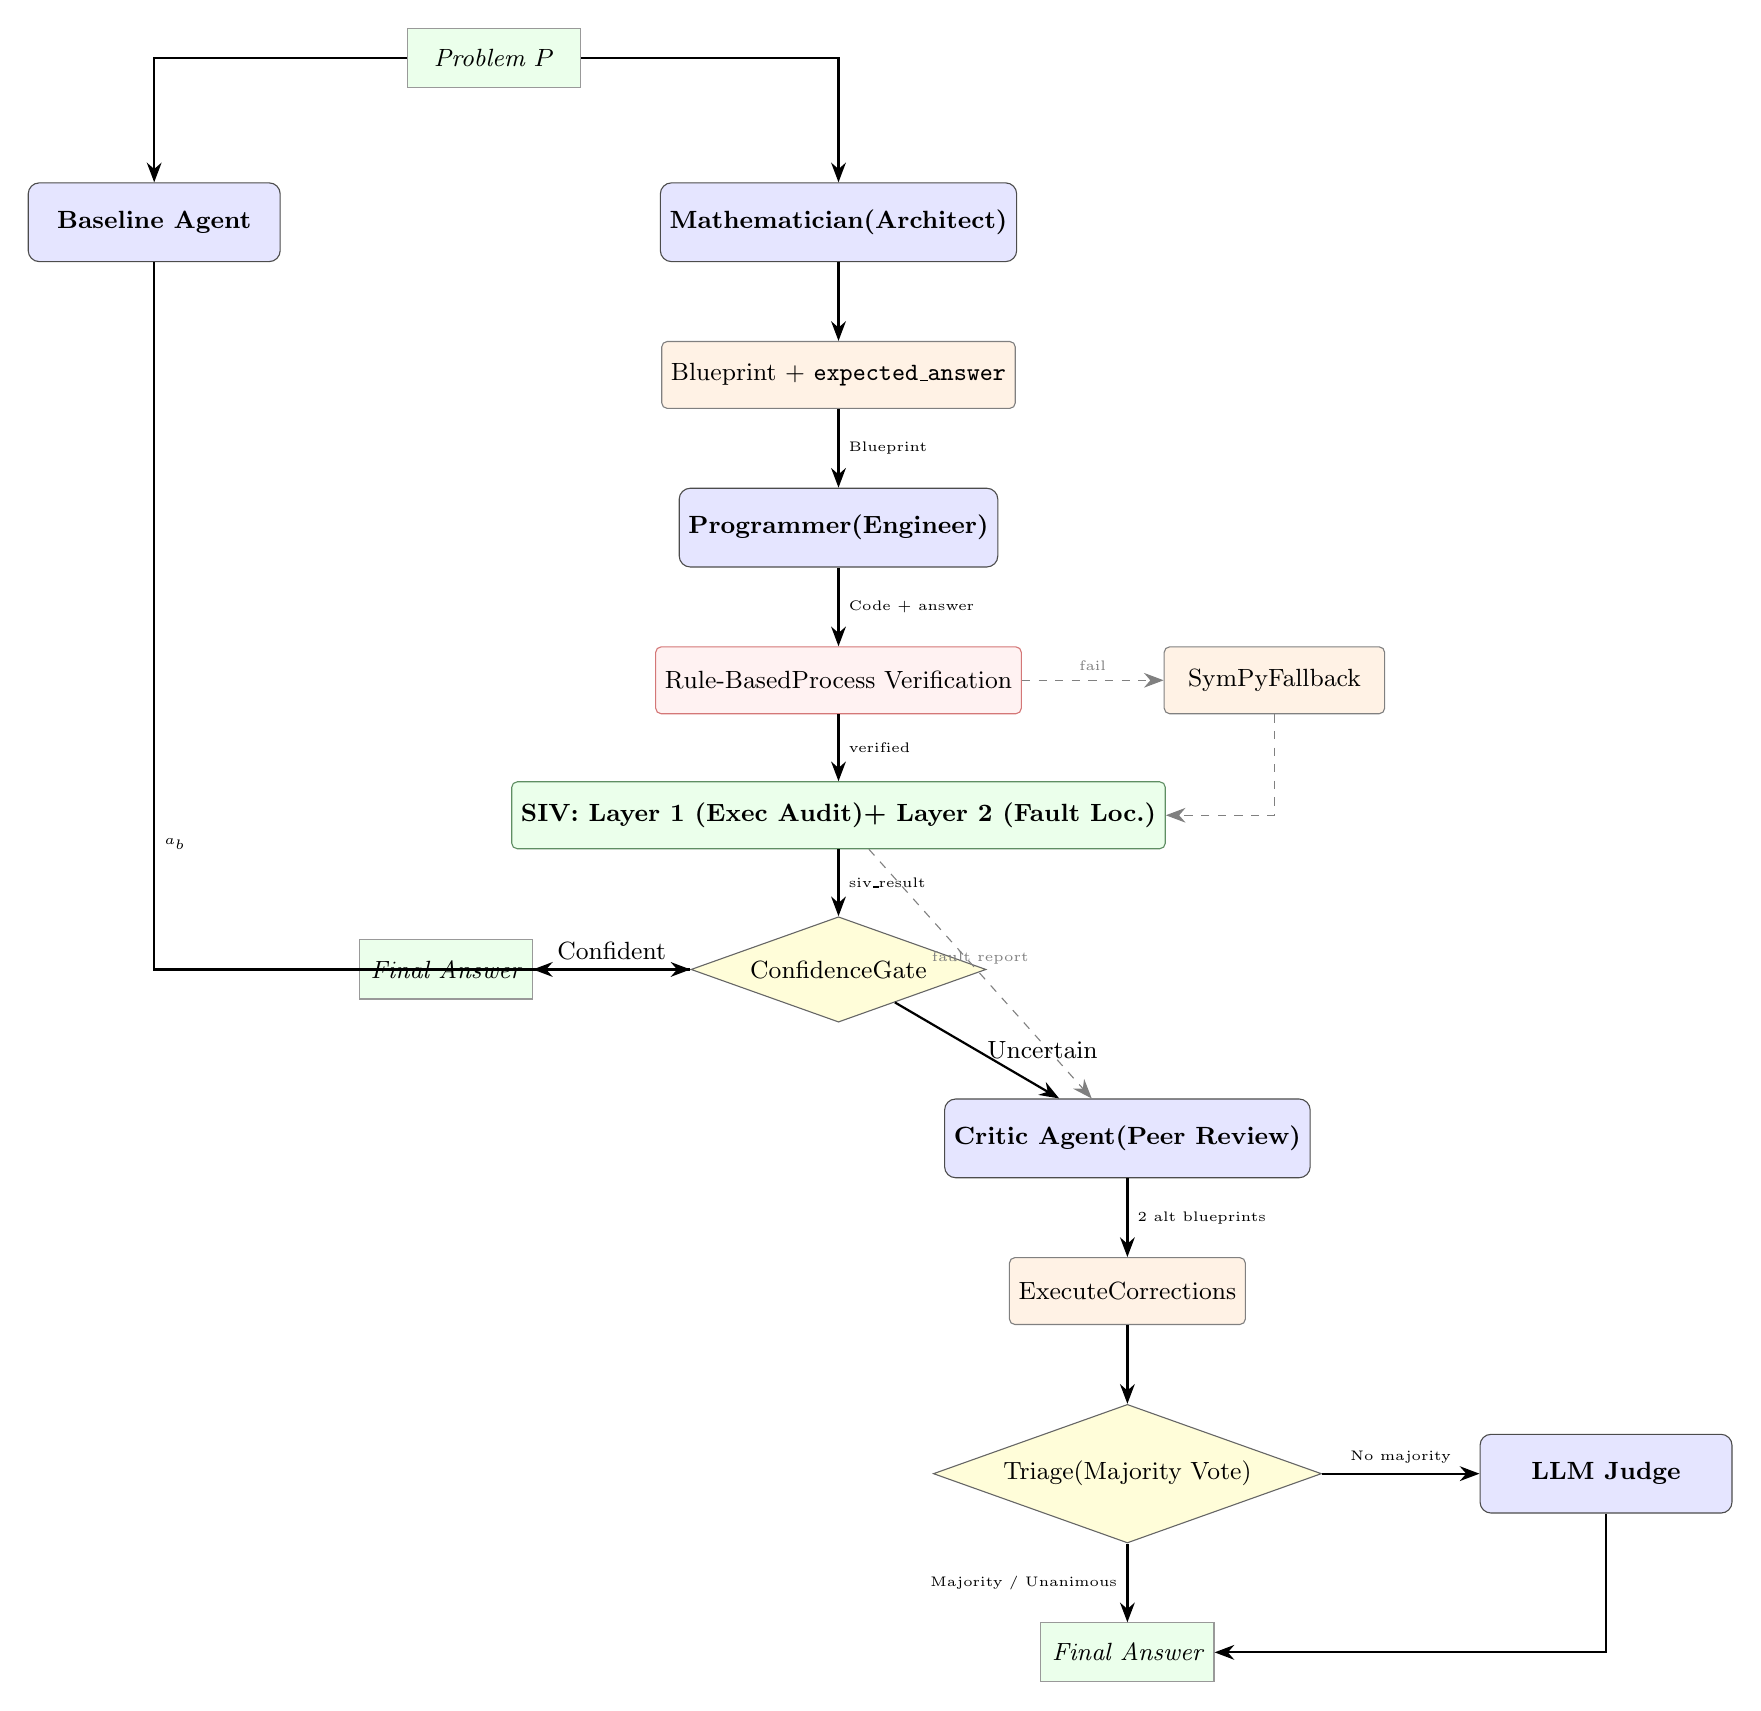
\begin{tikzpicture}[node distance=1.0cm and 1.9cm, auto]
    % Nodes
    \node[data] (input) {Problem $P$};
    \node[agent, below left=1.2cm and 1.6cm of input] (baseline) {Baseline Agent};
    \node[agent, below right=1.2cm and 1.0cm of input] (math) {Mathematician\\(Architect)};
    \node[process, below=of math] (blueprint) {Blueprint + \texttt{expected\_answer}};
    \node[agent, below=of blueprint] (prog) {Programmer\\(Engineer)};
    \node[verify, below=of prog] (verif) {Rule-Based\\Process Verification};
    \node[process, right=1.8cm of verif] (sympy) {SymPy\\Fallback};
    \node[siv_style, below=0.85cm of verif] (siv) {SIV: Layer 1 (Exec Audit)\\+ Layer 2 (Fault Loc.)};
    \node[decision, below=0.85cm of siv] (gate) {Confidence\\Gate};
    \node[data, left=2.0cm of gate] (output1) {Final Answer};
    \node[agent, below right=1.3cm and 0.4cm of gate] (critic) {Critic Agent\\(Peer Review)};
    \node[process, below=of critic] (exec2) {Execute\\Corrections};
    \node[decision, below=1.0cm of exec2] (triage) {Triage\\(Majority Vote)};
    \node[agent, right=2.0cm of triage] (judge) {LLM Judge};
    \node[data, below=1.0cm of triage] (output2) {Final Answer};
    % Arrows — primary path
    \draw[arrow] (input) -| (baseline);
    \draw[arrow] (input) -| (math);
    \draw[arrow] (math) -- (blueprint);
    \draw[arrow] (blueprint) -- node[right, font=\tiny]{Blueprint} (prog);
    \draw[arrow] (prog) -- node[right, font=\tiny]{Code + answer} (verif);
    \draw[arrowdashed] (verif) -- node[above, font=\tiny]{fail} (sympy);
    \draw[arrowdashed] (sympy) |- (siv);
    \draw[arrow] (verif) -- node[right, font=\tiny]{verified} (siv);
    \draw[arrow] (siv) -- node[right, font=\tiny]{siv\_result} (gate);
    \draw[arrowdashed] (siv) -- node[above, font=\tiny]{fault report} (critic);
    \draw[arrow] (baseline) |- node[below right, font=\tiny, pos=0.4]{$a_b$} (gate);
    \draw[arrow] (gate) -- node[above, font=\small]{Confident} (output1);
    \draw[arrow] (gate) -- node[right, font=\small]{Uncertain} (critic);
    \draw[arrow] (critic) -- node[right, font=\tiny]{2 alt blueprints} (exec2);
    \draw[arrow] (exec2) -- (triage);
    \draw[arrow] (triage) -- node[above, font=\tiny]{No majority} (judge);
    \draw[arrow] (triage) -- node[left, font=\tiny]{Majority / Unanimous} (output2);
    \draw[arrow] (judge) |- (output2);
\end{tikzpicture}
\caption{MAS-SHT pipeline (v10.0). Solid arrows show the primary execution path; dashed arrows show the SymPy fallback path and SIV fault localization report. SIV (green) performs a two-layer audit: Layer~1 (forward execution audit) detects Programmer deviations from the blueprint; Layer~2 (inverse fault localization) identifies which specific given variable is inconsistent. When the execution audit passes and all solvable givens reconstruct (confidence $\geq 0.90$), SHT is skipped; when inconsistencies are found, the fault report is forwarded to the Critic. \emph{Note:} SIV operates on the math$\to$math layer and cannot detect NL$\to$math translation errors. The baseline answer enters the triage pool with a fixed confidence of 0.5.}
\label{fig:architecture}
\end{figure}
% ----- 3.2 -----
\subsection{Stage 1: Zero-Shot Baseline}
\label{sec:baseline}
The baseline agent receives the problem $P$ with a minimal instruction to solve step-by-step and format the final answer as \texttt{ANSWER:~[[value]]}.
It serves two roles: providing a reference signal for the confidence gate (\Cref{sec:confidence_gate}) and acting as a last-resort fallback when the entire multi-agent pipeline fails.
Generation uses temperature $\tau=0.1$ and a 500-token budget.
\paragraph{Answer extraction.}
All agent outputs---including the baseline---pass through a three-stage extraction pipeline:
(1)~tagged extraction matching \texttt{ANSWER:~[[value]]},
(2)~last-number extraction scanning for the rightmost numeral (handling comma-separated values and stripping common unit suffixes such as ``dollars'', ``hours'', ``people''), and
(3)~pattern matching for common phrasings (e.g., ``the answer is 42'', ``result is 42'').
\paragraph{Error response guard.}
Before any extraction, an error-response guard (\texttt{\_is\_error\_response()}) checks whether the LLM returned an error string rather than a mathematical answer.
It detects responses prefixed with \texttt{ERROR\_} (covering \texttt{ERROR\_AUTH\_401}, \texttt{ERROR\_RATE\_LIMIT\_DAILY}, \texttt{ERROR\_BUDGET\_EXCEEDED}), HTTP status codes (401, 403, 429, 500--503) embedded in response text, and authentication or rate-limit phrasing.
This guard is applied at every point where a numeric answer is extracted in the pipeline, preventing HTTP codes from being parsed as mathematical answers---a subtle but critical failure mode identified during development.
% ----- 3.3 -----
\subsection{Stage 2: Mathematician Agent (Architect)}
\label{sec:mathematician}
The Mathematician receives the problem $P$ and a structured system prompt specifying a strict JSON output schema with six required fields:
\begin{itemize}[leftmargin=*,itemsep=2pt]
    \item \texttt{unknown}: a natural-language description of the target quantity.
    \item \texttt{givens}: a flat dictionary mapping descriptive variable names (e.g., \texttt{initial\_apples}) to their numeric values. Only values \emph{relevant} to the solution are included; distractors are explicitly excluded.
    \item \texttt{solution\_steps}: an ordered list of natural-language step descriptions.
    \item \texttt{equations}: an ordered list of valid Python-syntax expressions referencing the \texttt{givens} dictionary. The final equation must assign to \texttt{answer}.
    \item \texttt{expected\_answer}: a mental estimate of the numeric answer, obtained by tracing the equations with actual values before output.
    \item \texttt{distractor\_check}: explicit identification of any irrelevant numbers or context present in the problem statement.
\end{itemize}
\paragraph{Self-verification.}
The \texttt{expected\_answer} field serves a dual purpose.
First, the system prompt explicitly instructs the Mathematician to trace through its own equations with actual numbers before outputting the blueprint, and to revise them if the trace disagrees with its intuitive estimate.
This constitutes a within-call self-consistency check.
Second, \texttt{expected\_answer} is consumed downstream by the rule-based process verifier (\Cref{sec:verification}), acting as a cross-check independent of code execution.
\paragraph{Blueprint extraction cascade.}
The raw LLM response undergoes a four-stage extraction cascade:
(1)~direct JSON parsing of the full response after stripping markdown fences (\texttt{```json...```});
(2)~substring extraction by locating the outermost $\{\ldots\}$ brace pair;
(3)~field-level regex for the \texttt{givens} dictionary (\texttt{"\,givens"\,:\,\{...\}});
(4)~field-level regex for the \texttt{equations} array.
Stages 3--4 provide partial recovery even when the top-level JSON is broken.
Generation uses $\tau=0.0$ for maximum determinism and a 600-token budget.
\paragraph{Blueprint retry.}
If extraction yields an empty blueprint (no equations \emph{and} no givens), a single retry is issued using a simplified prompt that requests only the minimal required JSON fields.
In our experiments, this retry recovers approximately 30\% of initially failed blueprint generations.
Despite this mechanism, 37.8\% of problems in the hard-benchmark experiments still resulted in empty blueprint failures, representing the primary bottleneck of the pipeline.
% ----- 3.4 -----
\subsection{Stage 3: Programmer Agent (Engineer)}
\label{sec:programmer}
The Programmer receives the original problem $P$ and the blueprint formatted as a structured text block with labeled sections (\textsc{Target}, \textsc{Given Values}, \textsc{Solution Steps}, \textsc{Equations to Implement}, and optionally \textsc{Distractors to Ignore}).
This structured formatting, produced by a dedicated \texttt{format\_blueprint\_for\_programmer()} function, provides a cleaner interface than raw JSON and reduces misinterpretation.
The Programmer's system prompt enforces five strict rules:
(1)~initialize a \texttt{givens} dictionary with the exact values from the blueprint;
(2)~implement each blueprint equation in order;
(3)~store the final result in a variable named \texttt{answer};
(4)~print only the final numeric answer; and
(5)~use the exact variable names from the blueprint.
\paragraph{Sandboxed execution.}
Generated code is executed in a Python sandbox that blocks: \texttt{import os}, \texttt{import sys}, \texttt{subprocess}, \texttt{\_\_import\_\_}, \texttt{eval(}, \texttt{exec(}, \texttt{compile(}, \texttt{open(}, \texttt{file(}, \texttt{input(}, and \texttt{raw\_input()}.
Output is captured via \texttt{redirect\_stdout}, with fallback inspection of the \texttt{answer} and \texttt{result} local variables if no output was printed.
\paragraph{Repair loop.}
If execution fails, the specific error message is appended to the prompt as structured feedback:
\begin{quote}
\small\texttt{[Attempt 1] EXECUTION ERROR: NameError: 'step\_one' is not defined.\\
Check variable definitions.}
\end{quote}
The Programmer is re-prompted up to three times, each with accumulated feedback from all previous attempts.
Different error types receive tailored messages: \texttt{NameError} advises checking variable definitions, \texttt{KeyError} advises checking \texttt{givens} dict keys, and \texttt{ZeroDivisionError} is reported directly.
\paragraph{SymPy symbolic solver (fallback 1).}
When all repair attempts fail and the blueprint contains valid equations, the SymPy computer algebra system directly evaluates those equations.
The solver builds a restricted execution namespace from the \texttt{givens} dictionary, enriched with safe mathematical built-ins (\texttt{ceil}, \texttt{floor}, \texttt{sqrt}, \texttt{log}, \texttt{exp}, $\pi$).
Equations are executed sequentially via Python \texttt{exec}; for expressions that fail (e.g., due to unresolved variable references), the solver extracts the right-hand side, substitutes known values via string replacement, and attempts symbolic evaluation with \texttt{parse\_expr} (using implicit-multiplication transformations).
SymPy performs exact rational arithmetic, so this fallback is free of floating-point errors on correctly formulated equations.
The SymPy answer is assigned a confidence of 0.8 (vs.\ 1.0 for successful code execution), reflecting that correctness is still contingent on blueprint equation quality.
\paragraph{Performance when code succeeds.}
In our hard-benchmark experiments (\Cref{sec:results}), the Programmer successfully generated and executed code in 20 of 37 problems.
Remarkably, \emph{all 20 of these problems were answered correctly} (100\% accuracy).
This implies that the Architect--Engineer decomposition, when the blueprint is successfully constructed, is essentially sufficient for correctness---the full value of the pipeline lies in getting to a valid blueprint.
% ----- 3.5 -----
\subsection{Stage 3b: Rule-Based Process Verification}
\label{sec:verification}
After code execution produces an answer, a zero-API-call rule-based verifier performs four structural checks:
\begin{enumerate}[leftmargin=*,itemsep=2pt]
    \item \textbf{Givens consistency.}
    The \texttt{givens} dictionary is extracted from the code via AST pattern matching (\texttt{ast.literal\_eval} on the matched substring).
    Each key--value pair is compared against the blueprint's \texttt{givens}.
    Missing keys and numeric mismatches (tolerance $10^{-6}$) are flagged as critical issues.
    \item \textbf{Equation variable coverage.}
    For each equation in the blueprint, the left-hand side variable name is extracted and checked for presence in the code string.
    Missing variables indicate that the Programmer omitted or renamed a required computation step.
    \item \textbf{Answer sanity.}
    A negative answer is flagged unless the problem text contains keywords such as ``loss'', ``decrease'', ``debt'', ``below'', ``fewer'', or ``owe''.
    An answer exceeding the largest given value by a factor of $10^4$ is flagged as a magnitude anomaly.
    \item \textbf{Expected-answer cross-check.}
    If the blueprint's \texttt{expected\_answer} field is non-empty and the relative deviation of the code answer exceeds 10\%, a consistency warning is issued.
    The threshold of 10\% accommodates rounding but catches the most common arithmetic errors.
\end{enumerate}
Issues are classified as \emph{critical} (givens mismatch, negative answer, magnitude anomaly) or \emph{minor} (variable coverage gaps, expected-answer deviation).
When critical issues are found, the verifier confidence is reduced to $\max(0.3,\ 1.0 - 0.25 \cdot n_{\text{crit}} - 0.1 \cdot n_{\text{minor}})$, and a SymPy re-solve is attempted.
\paragraph{SymPy symbolic solver (fallback 2).}
If verification fails critically and SymPy produces a valid answer on the same blueprint, that answer replaces the Programmer's answer with a confidence of 0.75.
This second invocation point is distinct from the post-programmer-failure fallback (\Cref{sec:programmer}): here SymPy serves as an independent arithmetic check, potentially revealing that the equations are correct but the code contained a naming or syntax bug.
\paragraph{Verification in practice.}
In Experiment 1 ($n=37$), the rule-based verifier passed with confidence 1.0 on all 20 problems where the Programmer generated executable code.
This indicates that when code generation succeeds, the generated code faithfully implements the blueprint---the verifier's primary value is as a guard against regressions rather than a frequent corrective mechanism.
% ----- 3.6 -----
\subsection{Stage 3c: Symbolic Inverse Verification (SIV)}
\label{sec:siv}
\subsubsection{Motivation and Operating Scope}

After the Programmer (or SymPy fallback) produces a numeric answer, Symbolic Inverse Verification (SIV) performs a deterministic, zero-API-call audit using SymPy CAS.
SIV operates in two complementary layers targeting different failure modes.

\paragraph{What SIV verifies.}
SIV operates exclusively on the \emph{math$\to$math} execution layer.
It answers the question: \emph{did the Programmer faithfully execute the Architect's blueprint equations?}
Concretely, this covers: (i)~arithmetic deviations between the Programmer's code and the blueprint's symbolic chain; (ii)~ambiguities in the equation structure (non-uniquely invertible chains, multiple roots); and (iii)~unused given variables (declared in the blueprint but absent from the equation chain---potential distractors or missing equations).

\paragraph{What SIV cannot verify.}
SIV cannot detect errors in the \emph{NL$\to$math} translation layer---i.e., whether the Architect's blueprint correctly models the original problem.
If the Mathematician produces a blueprint with wrong equations that are nevertheless internally consistent, Layer~1 of SIV will pass (the Programmer executed those equations correctly) and Layer~2 will also pass (the givens reconstruct from the wrong answer via the wrong equations).
This is an explicit, irremovable scope limitation arising from SIV's design as a math$\to$math verifier.
We document it explicitly in the \texttt{SIVResult.verifies\_translation = False} field (always \textsc{False}) and in the generated fault localization reports.

\paragraph{Relationship to FOBAR.}
FOBAR \citep{jiang2024fobar} uses the LLM itself for backward verification, which gives it partial access to the NL$\to$math layer (the LLM can reason about whether the problem was modelled correctly) but is probabilistic and provides only a binary verdict.
SIV and FOBAR are therefore \emph{orthogonal}: FOBAR targets translation errors; SIV targets execution errors and provides per-variable fault localization.
Their combination is strictly stronger than either alone.

\subsubsection{Layer 1: Execution Audit (Forward)}

Layer~1 evaluates the blueprint equation chain in the \emph{forward} direction with all given values substituted numerically:
\[
  \texttt{blueprint\_answer} = \phi(g_1, g_2, \ldots, g_n)
\]
where $\phi$ is the closed-form SymPy expression for \texttt{answer} obtained by composing the blueprint equations, and $g_1,\ldots,g_n$ are the declared numeric givens.

The Layer~1 audit then checks:
\[
  \texttt{execution\_audit\_passed} = \left|\texttt{blueprint\_answer} - A\right| < \varepsilon
\]
where $A$ is the Programmer's computed answer and $\varepsilon$ is a combined absolute/relative tolerance ($10^{-6}$ absolute, $10^{-4}$ relative).

\paragraph{Interpretation.}
If \texttt{execution\_audit\_passed = True}, the Programmer's answer is consistent with what the blueprint equations produce when evaluated correctly.
If \texttt{execution\_audit\_passed = False}, the Programmer deviated from the blueprint: the computed answer does not match the forward evaluation of the declared equations, directly indicating a code-generation or execution error.

\paragraph{The tautology property.}
An important consequence of Layer~1 is that when \texttt{execution\_audit\_passed = True}, Layer~2 (inverse reconstruction) is \emph{guaranteed} to pass as well, because the Programmer's answer is the same value that the forward chain produces---and inverting a function to recover its own input is trivially consistent.
This means that in the \texttt{execution\_audit\_passed = True} regime, Layer~2 provides \emph{localization} of which specific given is recoverable, but not independent evidence of correctness.
The genuine diagnostic power of Layer~2 arises precisely when \texttt{execution\_audit\_passed = False}: the inverse reconstruction then identifies which given variable is most inconsistent with the deviating answer, guiding targeted Critic repair.

\subsubsection{Layer 2: Fault Localization (Inverse)}

Layer~2 operates in three steps:

\begin{enumerate}[leftmargin=*,itemsep=2pt]
    \item \textbf{Symbolic chain construction.} Each blueprint equation is parsed by SymPy with given variables treated as symbolic unknowns (e.g., \texttt{Symbol("initial\_apples", real=True)}). Equations are composed symbolically to produce a closed-form expression $\phi$ for \texttt{answer} as a function of all given variables.

    \item \textbf{Per-given inverse reconstruction.} For each given variable $g_i$ with original value $v_i$, all other givens are substituted with their numeric values, reducing $\phi$ to a univariate expression in $g_i$ alone. SymPy's \texttt{solve()} finds all real-valued roots of $\phi(g_i) = A$. All roots are collected and reported (not just the closest to $v_i$, to avoid a circular selection bias). A given is marked \emph{matched} if any root satisfies $|r - v_i| < \varepsilon_{\text{rel}}$ (relative tolerance $10^{-4}$). If multiple roots exist, the result is flagged \texttt{ambiguous = True} and all roots are reported.

    \item \textbf{Unused-given detection.} If a given variable $g_i$ does not appear in the free symbols of $\phi$, it is classified as an \emph{unused given}: declared in the blueprint but not contributing to the computation. These may be legitimate distractors correctly excluded by the Mathematician, or they may indicate a missing equation. SIV reports them in \texttt{unused\_givens} without marking them as failures, since their absence from the chain is ambiguous (correct exclusion vs.\ blueprint omission). This is a change from earlier versions that silently marked unused givens as matched.

    \item \textbf{Confidence and error localization.} Let $s$ be the number of solvable (chain-dependent) givens and $m \leq s$ the number that matched. The SIV localization confidence is $c = m / s$. If $c \geq 0.90$ \emph{and} \texttt{execution\_audit\_passed = True}, the solution is \emph{verified} at the execution level. The \texttt{failed\_givens} list names inconsistent variables; \texttt{get\_error\_localization\_report()} formats a targeted diagnostic covering both layers, forwarded verbatim to the Critic in Stage~5.
\end{enumerate}

\subsubsection{Special Cases}

\paragraph{Non-invertible chains.}
Equations involving \texttt{floor}, \texttt{ceiling}, absolute value, or conditional branches may not yield closed-form SymPy solutions.
In these cases, SIV reports \texttt{solvable = False} for those givens and abstains from penalizing the confidence, deferring to the rule-based verifier.
Coverage of the blueprint (what fraction of problems yield a fully invertible chain) is reported in \texttt{invertible}.

\paragraph{Multiple solutions (ambiguity).}
When SymPy returns multiple real roots (e.g., for quadratic equations), all roots are reported in \texttt{all\_real\_roots} and \texttt{ambiguous = True} is set.
A match is declared if \emph{any} root lies within tolerance of $v_i$, but the ambiguity is noted explicitly rather than concealed.
Prior versions selected the root closest to $v_i$, which was circular; the new design is transparent.

\paragraph{Unused givens.}
If a given does not appear in the symbolic chain, it is not solvable by inversion and is reported in \texttt{unused\_givens}.
It does not count toward $s$ (the solvable denominator) and does not reduce confidence.
The Critic prompt explicitly receives this list and is instructed to judge whether exclusion was intentional.

\subsubsection{Integration Points}

SIV integrates at three points in the pipeline:
\begin{enumerate}[leftmargin=*,itemsep=2pt]
    \item \textbf{Post-verification confidence.} If the execution audit passes (\texttt{execution\_audit\_passed = True}), rule-based verification concerns from Stage~3b may be overridden. This prevents the pipeline from discarding an answer that is execution-consistent merely due to minor code-style deviations caught by rule-based checks.

    \item \textbf{Confidence gate (highest-priority criterion, \Cref{sec:confidence_gate}).}
    SIV is evaluated as Criterion~0 in the gate.
    A result with \texttt{execution\_audit\_passed = True} \emph{and} \texttt{verified = True} \emph{and} confidence $\geq 0.90$ triggers a skip of SHT, saving 1--3 API calls.
    \texttt{execution\_audit\_passed = False} triggers a new gate reason (\texttt{siv\_execution\_error}) that activates SHT even when other criteria would pass.
    A result with a non-empty \texttt{failed\_givens} but \texttt{execution\_audit\_passed = True} triggers SHT with localization context.

    \item \textbf{SIV-informed Critic (\Cref{sec:sht}).}
    When SHT is triggered and SIV found specific inconsistencies (either execution error or failed given), the two-layer fault localization report is injected into the Critic's prompt as ``Automated Verification Report''.
    Layer~1 tells the Critic whether the Programmer deviated from the blueprint.
    Layer~2 tells the Critic which specific variable is inconsistent.
    This transforms the Critic's first alternative from speculative re-derivation into a targeted repair.
\end{enumerate}

% ----- 3.7 -----
\subsection{Stage 4: Confidence Gate}
\label{sec:confidence_gate}
The confidence gate is a deterministic, zero-cost component deciding whether to accept the primary answer or trigger hypothesis testing.
It evaluates criteria in priority order; any single trigger activates SHT:
\begin{enumerate}[leftmargin=*,itemsep=2pt]
    \item \textbf{SIV execution-consistent skip (Criterion 0a).} If the SIV execution audit passes \emph{and} all solvable givens reconstruct \emph{and} confidence $\geq 0.90$, the answer is accepted without SHT. This is the highest-priority positive signal. \emph{Note:} this criterion confirms execution fidelity only; NL$\to$math translation correctness is not verified.
    \item \textbf{SIV execution error (Criterion 0b).} If \texttt{execution\_audit\_passed = False} (the Programmer's answer deviates from the blueprint forward evaluation), SHT is triggered with reason \texttt{siv\_execution\_error}. This is a high-confidence negative signal---the Programmer deviated from the Architect's equations.
    \item \textbf{SIV fault localization (Criterion 0c).} If the chain is symbolically invertible but one or more solvable givens fail to reconstruct, SHT is triggered. The specific fault localization report is passed to the Critic (\Cref{sec:sht}).
    \item \textbf{Programmer failure.} The primary answer is ``unknown'' (all repair attempts and both SymPy invocations failed).
    \item \textbf{Baseline disagreement.} $|a_p - a_b| > 10^{-3}$ (numeric comparison) or string inequality (non-numeric answers).
    \item \textbf{Repair exhaustion.} The \texttt{quality\_metrics} dict reports \texttt{error = "Max attempts reached"}, indicating the Programmer produced code but failed to execute it successfully.
    \item \textbf{Negative answer.} $a_p < 0$ without linguistic support in the problem text.
    \item \textbf{Magnitude anomaly.} $|a_p| > 10^4 \times \max_{v \in \text{givens}} |v|$.
\end{enumerate}
An additional guard is applied: if $a_b = $ ``unknown'' as well as $a_p = $ ``unknown'', SHT is skipped (no reliable information source exists to anchor triage).
In our hard-benchmark experiments, the gate triggered on 94.6\% of problems.
The dominant reason is \textbf{baseline disagreement}: the Programmer's structured pipeline frequently produces a different answer from the zero-shot baseline, which may itself be unreliable on hard benchmarks.
This high trigger rate is not a failure of calibration but a reflection of genuine difficulty---on standard GSM8K, the trigger rate drops to 20\%.
% ----- 3.8 -----
\subsection{Stage 5: Critic-Based Structured Hypothesis Testing (SHT)}
\label{sec:sht}
\subsubsection{Design Rationale: Peer Review over Parallel Resampling}
A naive implementation of multi-hypothesis testing would instruct the same LLM to generate $k$ independent solutions and apply majority voting.
This has a fundamental statistical weakness: when the same model generates all candidates with different random seeds, the errors are \emph{correlated}.
A systematic misconception (e.g., confusing subtraction with division in a rate problem) recurs across all samples, rendering majority voting equivalent to a single draw from a biased distribution.
MAS-SHT addresses this with a \textbf{critic-based} design.
Rather than asking ``generate another solution'', the system asks ``what is wrong with this solution?''
This asymmetric framing forces metacognitive reasoning about failure modes before any correction is attempted.
\subsubsection{Critic Agent}
When the confidence gate triggers, a single LLM call to the Critic performs three tasks:
\begin{enumerate}[leftmargin=*,itemsep=2pt]
    \item \textbf{SIV-informed error diagnosis.} If SIV found specific inconsistencies, the Critic's prompt includes the full two-layer fault localization report (e.g., \emph{``Layer~1: Programmer's answer 120 deviates from blueprint evaluation 80 (rel\_error=0.50). Layer~2: variable \texttt{rate\_per\_hour} reconstructs as 12.0 from the answer, but problem states 8.0---check multiplication step''}). If SIV did not run or the chain was not invertible, the Critic reviews the primary solution against a standard five-point checklist: (a)~correct number extraction, (b)~absence of distractor contamination, (c)~correct mathematical operations, (d)~no missing steps, and (e)~whether the answer addresses the correct question.
    \item \textbf{Targeted correction.} The first alternative blueprint directly addresses the most likely error. Its \texttt{strategy\_name} records the error type (e.g., \texttt{correction\_of\_missing\_steps}, \texttt{correction\_of\_distractor\_inclusion}), providing interpretable diagnostic output. When SIV provides a specific failing variable, this correction is \emph{targeted} rather than speculative.
    \item \textbf{Independent rederivation.} The second alternative blueprint solves the problem from scratch without reference to the primary approach, using \texttt{strategy\_name = independent\_rederivation}.
\end{enumerate}
The Critic outputs a JSON object with a \texttt{review} field and an \texttt{alternatives} array of exactly two blueprints.
Generation uses $\tau=0.3$, permitting variation in error diagnosis while maintaining structural JSON fidelity.
\subsubsection{Baseline as an Active Triage Candidate}
Crucially, the zero-shot baseline answer is not merely a gate trigger---it is registered as a triage candidate with a fixed confidence of 0.5.
This means that if both the Programmer's code and the Critic's alternatives fail to execute, the baseline answer can still be selected by the Judge as the best available answer.
This architectural choice ensures the triage pool always contains at least two candidates (primary + baseline) and that no information is discarded.
\subsubsection{Alternative Execution}
Each of the Critic's two alternative blueprints is passed to the Programmer for a single execution attempt (no repair loop, to bound API costs).
Combined with the primary answer and the baseline, this yields up to four candidates.
\subsubsection{Triage (Majority Voting)}
Candidates are filtered to those with \texttt{code\_success = True} and a non-null parsed numeric answer, then grouped by answer value (tolerance $\epsilon = 10^{-3}$).
Groups are ranked by size, with average confidence as a tiebreaker.
Three outcomes are possible:
\begin{itemize}[leftmargin=*,itemsep=2pt]
    \item \textbf{Unanimous}: all valid candidates share a single answer $\Rightarrow$ accepted directly.
    \item \textbf{Majority}: the largest group has $\geq 2$ members and strictly dominates $\Rightarrow$ accepted.
    \item \textbf{No majority}: candidates disagree without a dominant group $\Rightarrow$ escalate to the LLM Judge.
\end{itemize}
\subsubsection{LLM Judge}
When triage fails, the Judge receives all candidate summaries (strategy name, execution status, equations, and first 300 characters of code) and selects the most reliable answer.
The Judge evaluates: (1)~code execution success, (2)~mathematical correctness of equations, (3)~completeness, (4)~inter-candidate agreement, and (5)~simplicity.
The Judge uses $\tau=0.0$ and outputs \texttt{SELECTED\_ANSWER:~[[value]]} and \texttt{SELECTED\_STRATEGY:~[[name]]} in a structured format.
\paragraph{API call budget.}
\Cref{tab:api_calls} summarizes the API call budget across execution paths with observed frequencies from Experiment 1.
The most frequent paths are SHT with no productive alternative blueprints (4 calls, 45.9\%) and SHT with Judge resolution (5 calls, 45.9\%), yielding an observed average of 4.46 calls per problem.
When SIV verifies execution consistency (confident skip), only 3 calls are used, saving at least 1 additional call per verified problem.
\begin{table}[h]
\centering
\caption{API calls per problem across execution paths. Observed frequencies from Experiment 1 ($n=37$, Qwen3-32B). SIV-consistent skip (3 calls) occurs when SIV execution audit passes and all solvable givens reconstruct.}
\label{tab:api_calls}
\begin{tabular}{p{5.8cm}ccc}
\toprule
\textbf{Path} & \textbf{Calls} & \textbf{Condition} & \textbf{Observed} \\
\midrule
Confident skip (SIV exec-consistent / no SHT)    & 3 & SIV exec.$+$loc.$\geq$0.90      & 5.4\% \\
SHT + no alt.\ produced           & 4 & Critic fails; 2-cand.\ unanimous      & 45.9\% \\
SHT + Judge                       & 5 & Gate fails; no majority               & 45.9\% \\
SHT + Majority (full candidates)  & 6 & Gate fails; majority found            & 2.7\% \\
\midrule
\textbf{Average} & \textbf{4.46} & & \\
\bottomrule
\end{tabular}
\end{table}
% ----- 3.9 -----
\subsection{Heterogeneous Model Configuration}
\label{sec:heterogeneous}
MAS-SHT supports assigning different LLMs to different agent roles via an \texttt{AgentRole} enum (\textsc{Baseline}, \textsc{Mathematician}, \textsc{Programmer}, \textsc{Hypothesis\_Generator}, \textsc{Judge}) and a \texttt{ModelConfig} dataclass specifying provider and model name.
Five pre-defined presets are available:
\begin{itemize}[leftmargin=*,itemsep=1pt]
    \item \textit{homogeneous\_groq}: all roles use Qwen3-32B.
    \item \textit{diverse\_groq}: LLaMA~3.3~70B (Mathematician, Programmer, Judge), Gemma~2~9B (Baseline), Mixtral~8$\times$7B (Critic).
    \item \textit{cross\_provider}: Groq LLaMA~70B for structured roles, Google Gemini~2.5~Flash-Lite for Baseline and Critic.
    \item \textit{budget\_optimized}: LLaMA~8B for Baseline and Programmer, 70B for Mathematician, Critic, and Judge.
    \item \textit{homogeneous\_google}: all roles use Gemini~2.5~Flash-Lite.
\end{itemize}
Client deduplication ensures that roles sharing the same (provider, model) pair share a single connection object, avoiding redundant authentication overhead.
Our primary experiments use the \textit{homogeneous\_groq} preset with Qwen3-32B.
% ----- 3.10 -----
\subsection{Distractor Hardening}
\label{sec:hardener}
When distractor hardening is enabled, 1--3 sentences are appended to each problem statement.
Each sentence introduces a random numeric value, person name, and item, explicitly flagged as irrelevant (e.g., \emph{``Unrelated note: Alex counted 42 stickers yesterday, but that does not affect the question.''}).
The distractor values are drawn from uniform distributions ($n_1 \in [7, 99]$, $n_2 \in [10, 250]$, $n_3 \in [2, 60]$), and names and items are sampled from fixed pools.
The Mathematician's \texttt{distractor\_check} field explicitly identifies these values, and the \texttt{givens} dictionary is supposed to exclude them.
SIV provides an additional safeguard: if a distractor value was inadvertently included in \texttt{givens}, it would appear in Layer~2's \texttt{unused\_givens} list (since the equations do not actually use it to produce the answer), flagging it in the Critic's fault localization report.
All Experiment 1 evaluations use distractor hardening.
% ----- 3.11 -----
\subsection{Implementation Robustness}
\label{sec:robustness}
Several engineering decisions are critical for reliable operation under free-tier API constraints.
\paragraph{Rate limiting.}
Two independent rate limiters operate at the provider level: 12 RPM for Groq (constrained by the $\sim$6K tokens/min TPM limit for 32B models) and 15 RPM for Google.
Each limiter enforces its inter-call delay using a thread-safe lock, allowing concurrent requests from multiple agents to be serialized safely.
An additional inter-problem cooldown of 3 seconds (with SHT enabled) or 2 seconds (without) prevents token bursts across problems.
\paragraph{Token budget management.}
A daily token budget of 100,000 tokens (Groq free tier) is tracked in real time.
The \emph{estimation formula} is:
\begin{equation*}
\hat{T} = \left\lfloor \frac{|\text{input\_chars}|}{4} \right\rfloor + \lfloor 0.35 \times \text{max\_tokens} \rfloor
\end{equation*}
This realistic estimate (models rarely consume their full \texttt{max\_tokens} allocation) prevents the premature budget exhaustion that would occur with pessimistic worst-case budgeting.
Actual token usage is recorded from the API response's \texttt{usage.total\_tokens} field when available.
If the remaining budget falls below a per-problem threshold (9,000 tokens with SHT, 4,500 without), processing stops gracefully.
\paragraph{Retry and backoff policy.}
Each LLM call attempts up to 4 times (reduced from 6 in v9.0 to avoid cascading backoffs).
Authentication errors (HTTP 401, 403) are non-retryable and return immediately with a prefixed error code.
Rate limit errors (HTTP 429) extract the wait duration from Groq's error format (\texttt{"try again in Xm Y.Zs"}) and sleep for the exact requested duration plus a 5-second buffer.
If the extracted wait exceeds 600 seconds, the problem is classified as a daily-limit hit and processing stops.
Generic failures use exponential backoff with jitter: $\min(120,\ 2^{\text{attempt}} \times 5 + \mathcal{U}(0, 5))$ seconds.
\paragraph{Response caching.}
All LLM calls are optionally cached using an MD5 hash of the (provider, model, messages, temperature) tuple as key.
The cache is persisted to disk as a pickle file (\texttt{call\_cache\_v6.pkl}) and reloaded at startup, enabling deterministic re-runs of experiments without additional API costs.
\paragraph{Consecutive failure detection.}
During a pipeline run, if five consecutive problems both return ``unknown'' for baseline and MAS answers, execution aborts with a diagnostic message, preventing silent failure accumulation when an API key expires or service goes offline.
% ============================================================
\section{Experimental Setup}
\label{sec:experiments}
% ============================================================
\subsection{Benchmarks}
We evaluate on five mathematical reasoning benchmarks:
\begin{itemize}[leftmargin=*,itemsep=3pt]
    \item \textbf{GSM8K} (test split) \citep{cobbe2021gsm8k}: 1,319 grade-school math problems requiring 2--8 reasoning steps.
    \item \textbf{GSM-Hard} \citep{gao2023pal}: GSM8K problems with numbers replaced by larger values; correct answers can be in the millions, testing numerical robustness.
    \item \textbf{GSM-Plus} \citep{li2024gsmplus}: Systematic perturbations of GSM8K covering eight types: digit expansion, distraction insertion, reversing operations, adding operations, numerical substitution, and others.
    \item \textbf{GSM-Symbolic (P2)} \citep{shi2023gsmsymbolic}: The hardest complexity level, combining symbolic value variations with additional problem clauses.
    \item \textbf{SVAMP} \citep{patel2021svamp}: Structurally varied arithmetic problems from diverse sources, testing cross-domain generalization.
\end{itemize}
\subsection{Language Models and Infrastructure}
\paragraph{Experiment 1 (Hard Benchmarks).}
All five benchmarks are sampled with distractor hardening enabled.
All agent roles use \textbf{Qwen3-32B} via the Groq inference API (homogeneous preset).
Groq provides low-latency access under a free-tier constraint of approximately 100,000 tokens/day at 12 RPM.
\paragraph{Experiment 2 (Standard GSM8K).}
A second run on 10 standard GSM8K problems (no distractor hardening) uses the SambaNova inference API, verifying that the framework generalizes across inference providers.
\paragraph{Note on SIV evaluation.}
The experiments reported in \Cref{sec:results} were conducted under v9.1 of the pipeline (prior to the integration of SIV in v10.0).
SIV metrics therefore appear as \texttt{null} in the experiment logs.
Quantitative evaluation of SIV's two-layer impact---specifically, the execution audit catch rate, the rate at which SIV correctly skips SHT on execution-consistent problems, and the degree to which its fault localization report improves Critic corrections---is reserved for future experiments using v10.0.
\subsection{Temperature and Token Settings}
Role-specific temperatures: $\tau=0.0$ (Mathematician, Judge), $\tau=0.05$ (Programmer), $\tau=0.1$ (Baseline), $\tau=0.3$ (Critic).
Token budgets (v9.1 reduced settings): Baseline and Judge 500 tokens, Mathematician 600 tokens, Programmer 1000 tokens, Critic 900 tokens.
\subsection{Evaluation Metrics}
\paragraph{Accuracy.}
A prediction is correct if the extracted numeric answer matches the gold answer within $\epsilon=10^{-3}$.
Gold answers use the \texttt{\#\#\#\#} delimiter format standard in GSM8K; SVAMP and GSM-Plus provide direct numeric fields.
\paragraph{SHT-specific metrics.}
Trigger rate, rescue count (baseline wrong $\to$ MAS correct), damage count (baseline correct $\to$ MAS wrong), net benefit, and triage method distribution.
\paragraph{Solver path metrics.}
Fraction of problems resolved by Programmer (optimized), empty blueprint, Programmer (failed after repairs), and SymPy fallback.
% ============================================================
\section{Results}
\label{sec:results}
% ============================================================
\subsection{Overall Accuracy}
\Cref{tab:main_results} presents the main accuracy comparison.
The most striking finding is the magnitude of improvement on hard benchmarks: the zero-shot baseline achieves only 5.4\% accuracy with Qwen3-32B, while MAS-SHT reaches 56.8\%---a gain of \textbf{+51.4 percentage points}.
On standard GSM8K (Experiment 2), the baseline achieves 90\% and MAS-SHT reaches 100\%, confirming the framework also avoids regressions on easier problems.
\begin{table}[h]
\centering
\caption{Accuracy comparison. Experiment 1: Qwen3-32B on a hard mixed-benchmark set ($n=37$) with distractor hardening. Experiment 2: SambaNova on GSM8K standard ($n=10$, no distractor hardening).}
\label{tab:main_results}
\begin{tabular}{lcccc}
\toprule
\textbf{Experiment} & \textbf{Model} & \textbf{Baseline} & \textbf{MAS+SHT} & \textbf{$\Delta$} \\
\midrule
Hard mix (Exp.~1)     & Qwen3-32B   & 5.4\%   & 56.8\%  & +51.4 pp \\
GSM8K std.\ (Exp.~2)  & SambaNova   & 90.0\%  & 100.0\% & +10.0 pp \\
\bottomrule
\end{tabular}
\end{table}
\subsection{Per-Benchmark Performance (Experiment 1)}
\Cref{tab:per_benchmark} shows per-benchmark accuracy on Experiment 1.
Baseline accuracy is near zero across all hard benchmarks.
MAS-SHT consistently outperforms the baseline, with the largest gains on GSM-Plus (83.3\%) and GSM-Hard (62.5\%).
GSM-Symbolic P2 is the most challenging (37.5\%), reflecting the additional complexity clauses that make blueprint construction difficult even with the retry mechanism.
\begin{table}[h]
\centering
\caption{Per-benchmark accuracy, Experiment 1 (Qwen3-32B, $n=37$ total, distractor hardening).}
\label{tab:per_benchmark}
\begin{tabular}{lcccc}
\toprule
\textbf{Benchmark} & \textbf{$n$} & \textbf{Baseline} & \textbf{MAS+SHT} & \textbf{$\Delta$} \\
\midrule
GSM-Hard            & 8  & 0.0\%   & 62.5\%  & +62.5 pp \\
SVAMP               & 8  & 12.5\%  & 62.5\%  & +50.0 pp \\
GSM8K (hard sample) & 7  & 0.0\%   & 42.9\%  & +42.9 pp \\
GSM-Plus            & 6  & 16.7\%  & 83.3\%  & +66.7 pp \\
GSM-Symbolic P2     & 8  & 0.0\%   & 37.5\%  & +37.5 pp \\
\midrule
\textbf{Overall}    & 37 & 5.4\%   & 56.8\%  & +51.4 pp \\
\bottomrule
\end{tabular}
\end{table}
\subsection{Solver Path Distribution and Code-Execution Accuracy}
\Cref{tab:solver_agents} shows the distribution of solver paths and their per-path accuracy.
The most important finding is that \textbf{the Programmer achieves 100\% accuracy on all 20 problems where it successfully generates and executes code}.
This demonstrates that the Architect--Engineer blueprint mechanism, when operative, effectively constrains code generation to produce correct computations.
In contrast, problems where the Mathematician fails to produce a parseable blueprint (\textit{empty blueprint}, 37.8\%) achieve only 7.1\% accuracy---a single rescue by the Judge from among 14 failed blueprints.
This confirms that blueprint construction quality is the \emph{sole bottleneck} of the pipeline: the downstream stages (code execution, verification, SHT) function correctly whenever they receive valid input.
\begin{table}[h]
\centering
\caption{Solver path distribution and per-path accuracy, Experiment 1 ($n=37$).}
\label{tab:solver_agents}
\begin{tabular}{lccc}
\toprule
\textbf{Solver Path} & \textbf{Count} & \textbf{Fraction} & \textbf{MAS Accuracy} \\
\midrule
Programmer (successful)         & 20 & 54.1\% & \textbf{100.0\%} \\
Programmer (empty blueprint)    & 14 & 37.8\% & 7.1\%   \\
Programmer (failed after repairs) & 3 &  8.1\% & 0.0\%   \\
\midrule
\textbf{Overall}                & 37 & 100\%  & 56.8\%  \\
\bottomrule
\end{tabular}
\end{table}
\subsection{Structured Hypothesis Testing Analysis}
\Cref{tab:sht_analysis} provides a detailed breakdown of SHT behavior.
\begin{table}[h]
\centering
\caption{SHT analysis, Experiment 1 ($n=37$).}
\label{tab:sht_analysis}
\begin{tabular}{lcc}
\toprule
\textbf{Metric} & \textbf{Value} & \textbf{Fraction} \\
\midrule
SHT Triggered             & 35 & 94.6\% \\
\quad Confident skip      &  2 &  5.4\% \\
\midrule
\multicolumn{3}{l}{\textit{Triage breakdown among triggered ($n=35$)}} \\
\quad Unanimous           & 17 & 48.6\% \\
\quad Judge               & 17 & 48.6\% \\
\quad Majority            &  1 &  2.9\% \\
\midrule
MAS Correct (triggered)   & 19/35 & 54.3\% \\
MAS Correct (confident skip) & 2/2 & 100\% \\
\midrule
Rescue count (baseline $\times$ $\to$ MAS $\checkmark$) & 19 & --- \\
Damage count  (baseline $\checkmark$ $\to$ MAS $\times$) &  0 & --- \\
\textbf{Net benefit}      & \textbf{+19} & --- \\
\bottomrule
\end{tabular}
\end{table}
\paragraph{Zero damage.}
In all 37 problems, MAS-SHT never changed a correct baseline answer to an incorrect one.
This is a strong safety property: the framework is monotonically beneficial in these experiments.
\paragraph{High trigger rate.}
The 94.6\% trigger rate (vs.\ 20\% on standard GSM8K) confirms that the confidence gate correctly identifies problem difficulty.
The primary trigger is baseline disagreement: the Programmer's structured approach often produces a different answer from the zero-shot baseline, which on hard benchmarks is itself unreliable.
\paragraph{Judge-heavy resolution.}
Among triggered cases, 48.6\% required the Judge.
This high rate arises from the \emph{empty blueprint} failure mode: when the Mathematician fails, the Critic's alternatives also fail code execution, leaving only the primary (``unknown'') and the baseline as valid candidates---a two-way disagreement that triage cannot resolve by majority.
In these cases, the Judge evaluates the reasoning quality of the baseline against the failed attempts and typically selects the baseline answer, which explains the 7.1\% accuracy on empty-blueprint problems.
\paragraph{Majority triage.}
Only 1 of 35 triggered cases was resolved by majority vote (\textit{gsm-hard\_243}: the Critic's \texttt{correction\_of\_missing\_steps} blueprint produced 161,868.2, agreeing with the primary, while the baseline had 323,736.4 and the independent rederivation also produced the correct value, giving a 3-candidate majority).
\subsection{Confidence Gate Trigger Analysis}
\Cref{tab:gate_reasons} shows the estimated trigger reason distribution.
Baseline disagreement dominates strongly, confirming its value as a calibration signal.
\begin{table}[h]
\centering
\caption{Estimated distribution of confidence gate trigger reasons, Experiment 1.}
\label{tab:gate_reasons}
\begin{tabular}{lc}
\toprule
\textbf{Trigger Reason} & \textbf{Proportion (est.)} \\
\midrule
Baseline disagreement ($a_p \neq a_b$) & $\sim$60--70\% \\
Programmer failure ($a_p = $ ``unknown'') & $\sim$25--35\% \\
Negative answer / magnitude anomaly        & $<5\%$ \\
\bottomrule
\end{tabular}
\end{table}
\subsection{Process Verification in Practice}
In Experiment 1, the rule-based verifier passed with confidence 1.0 on all 20 code-execution successes.
No verification failure triggered the SymPy post-verification fallback during these runs.
This indicates that when the Programmer successfully generates executable code, it faithfully replicates the blueprint's \texttt{givens} and equations without structural violations.
\subsection{Distractor Robustness}
Distractor hardening was applied to all Experiment 1 problems.
The Mathematician's \texttt{distractor\_check} field correctly identified distractor values in the majority of successfully constructed blueprints.
GSM-Plus distraction insertion variants achieved 100\% accuracy (2/2 problems), the highest per-type accuracy across all GSM-Plus perturbation categories, suggesting the explicit distractor checklist in the blueprint schema is particularly effective at preventing contamination.
% ============================================================
\section{Discussion}
\label{sec:discussion}
% ============================================================
\subsection{Blueprint Construction as the Sole Bottleneck}
The most important empirical finding of this work is precise: MAS-SHT achieves \emph{100\% accuracy when the Programmer generates valid executable code}.
All 21 wrong answers in Experiment 1 originate from problems where the Mathematician either failed to produce parseable JSON (14 cases) or produced an empty blueprint despite the retry (3 additional cases).
This finding sharply delineates the research agenda: improving the downstream pipeline (verification, SHT, Judge) yields diminishing returns; improving blueprint construction yields proportional accuracy gains.
Empty blueprints arise primarily in two scenarios:
\textit{(i)} complex multi-clause problems (GSM-Symbolic P2 contributes 5 of the 14 empty blueprints) where the model exhausts its 600-token budget writing reasoning prose before emitting JSON; and
\textit{(ii)} problems requiring non-trivial mathematical structuring (percentages, proportions, inverse rates) where the model fails to identify a clean Python-expressible equation chain.
The token budget cap is thus an active constraint: increasing it from 600 to 1000 may recover a substantial fraction of empty-blueprint failures.
\subsection{Correlated Errors and the Critic Design}
A central architectural decision in v9.0 was replacing the ``5 strategy archetypes'' parallel generation approach with critic-based peer review.
Under the original design, the same model was instructed to generate two alternative blueprints from different mathematical archetypes (Arithmetic-Sequential, Algebraic-Equational, Unit-Rate, Working-Backwards, Partitioning).
In practice, however, correlated errors dominated: the same misidentified variable or incorrect operation appeared in all alternatives, because the model's systematic misconception about the problem was not affected by the archetype constraint.
Majority voting over correlated candidates is provably no better than selecting a single random candidate.
The critic design introduces a qualitatively different cognitive demand: the model must first articulate \emph{what is wrong} before generating a correction.
This metacognitive framing partially breaks correlation because the model must commit to a specific failure hypothesis---and different failure hypotheses lead to structurally different corrections.
The interpretable \texttt{strategy\_name} values observed in our data (e.g., \texttt{correction\_of\_missing\_steps} in the one majority-resolution case) confirm that the Critic does identify distinct, actionable errors rather than merely rephrasing the primary approach.
\subsection{Symbolic Inverse Verification: Two-Layer Design and Scope}

SIV introduces a two-layer deterministic audit that targets the \emph{execution layer} of the Architect--Engineer pipeline.

\paragraph{Layer~1 (Execution Audit) as the primary signal.}
The most direct contribution of Layer~1 is detecting when the Programmer's computed answer deviates from what the blueprint equations actually evaluate to.
This is a necessary precondition for any meaningful inverse reasoning: if the Programmer's answer does not match the forward evaluation of the blueprint, the execution is incorrect regardless of whether the blueprint itself is correct.
Layer~1 is the first check that runs and sets the interpretation frame for Layer~2.

\paragraph{Layer~2 (Fault Localization) as the Critic enabler.}
When Layer~1 detects an execution deviation, Layer~2 identifies precisely which declared given variable is inconsistent with the deviating answer.
This per-variable diagnosis is the primary novel contribution relative to FOBAR \citep{jiang2024fobar}: FOBAR produces a binary pass/fail verdict, whereas SIV produces a named fault report (\texttt{failed\_givens}, \texttt{all\_real\_roots}, \texttt{ambiguous}) that the Critic can act on directly.
This transforms the Critic's first alternative from speculative re-derivation into targeted repair.

\paragraph{The tautology property and why Layer~2 is honest about it.}
When Layer~1 passes (\texttt{execution\_audit\_passed = True}), the Programmer's answer is exactly what the blueprint equations compute, which means Layer~2's inverse reconstructions are \emph{guaranteed} to pass---they are algebraic rearrangements of the same expression.
This is not a failure of SIV; it is an inherent property of any math$\to$math verifier.
We address this by: (i)~making the execution audit the explicit primary signal; (ii)~capping SIV confidence below 1.0 even on full reconstruction ($\leq 0.97$) to reflect that the NL$\to$math layer is untested; and (iii)~documenting the limitation in \texttt{verifies\_translation = False}.

\paragraph{Explicit scope: NL$\to$math errors are outside SIV's detection range.}
SIV cannot detect a blueprint that correctly executes the wrong equations---i.e., a blueprint that models the problem incorrectly but is internally consistent.
This is the translation layer, and it is FOBAR's comparative advantage.
The correct architectural response is \emph{composition}: use SIV for execution-layer audit and fault localization, and use a separate NL-layer verifier (LLM-based or human) for translation correctness.
Future work should evaluate whether adding a lightweight FOBAR-style check as an additional confidence gate criterion improves accuracy beyond either method alone.

\paragraph{Additional scope flags.}
Two further limitations are explicitly encoded in the implementation.
(i)~\emph{Non-invertible chains}: equations with \texttt{floor}, \texttt{ceiling}, absolute value, or conditional branches may not yield closed-form SymPy solutions; SIV abstains for those variables.
(ii)~\emph{Empty blueprints}: when the Mathematician fails (37.8\% of Experiment~1), SIV cannot run at all, which is precisely the regime where verification is most needed.

\subsection{The Baseline as an Active Triage Participant}
A subtle but important design choice is registering the zero-shot baseline answer as a triage candidate with a fixed confidence of 0.5.
This choice has two effects.
First, on problems where both the primary and the Critic's alternatives fail code execution, the baseline answer alone can achieve a ``unanimous'' triage outcome (two failed candidates plus baseline), which the Judge then confirms or overrides.
This explains the high Judge rate (48.6\%): the Judge is not called because candidates \emph{disagree}, but because only the baseline is a ``valid'' candidate in the triage sense.
Second, on standard benchmarks where the baseline is highly reliable, its participation in triage provides additional confirmation of correct answers, potentially reducing false SHT triggers.
\subsection{The Role of the SymPy Fallback}
Although SymPy was not invoked as the final solver in any of the 37 Experiment 1 problems, it plays two structural roles that are difficult to quantify from these results alone.
First, as a post-programmer-failure fallback (confidence 0.8), it provides a backstop against code generation failures when the blueprint equations are correct---a scenario that did not occur in these experiments but is expected to arise on different problem distributions.
Second, as a post-verification fallback (confidence 0.75), it provides arithmetic confirmation that the blueprint's equations are correctly specified even when the code implementation has bugs.
The 100\% verification pass rate in Experiment 1 means SymPy was not needed, but this cannot be assumed to generalize.
\subsection{API Cost Analysis}
The observed average API call count per problem in Experiment 1:
\begin{equation*}
\bar{c} = 0.054 \times 3 + 0.459 \times 4 + 0.459 \times 5 + 0.027 \times 6 = 4.46 \text{ calls/problem}
\end{equation*}
At an accuracy gain of +51.4 percentage points, this is approximately $4.46 / 51.4 \approx 0.087$ additional API calls per percentage point gained---highly cost-effective.
SIV introduces \emph{zero} additional API calls, meaning any problems it correctly verifies (skipping SHT) \emph{reduce} the average call count.
\subsection{Limitations}
\paragraph{Sample size.}
Experiments use $n=37$ and $n=10$ problems, limited by the Groq free-tier budget.
While results are internally consistent, statistical significance testing and confidence intervals are not reliable at these sample sizes.
Larger-scale evaluation is essential to confirm per-benchmark trends.
\paragraph{Blueprint bottleneck.}
The 37.8\% empty-blueprint failure rate caps MAS-SHT's theoretical accuracy at approximately 62\% even with perfect downstream processing---the per-benchmark results are consistent with this ceiling.
\paragraph{SIV not yet evaluated empirically.}
The Symbolic Inverse Verification module was integrated in v10.0 after the experiments reported here.
Quantitative measurement of SIV's effect on execution error detection rate, SHT trigger rate reduction, Critic correction quality, and overall accuracy remains as future work.
The explicit scope limitation (NL$\to$math errors are undetectable) will need to be quantified empirically by measuring the fraction of errors that are execution-layer vs.\ translation-layer in nature.
\paragraph{Benchmark scope.}
All five benchmarks are arithmetic word problems.
Extension to algebra, geometry, combinatorics, probability, and calculus requires structural modifications to the blueprint schema (e.g., supporting inequality constraints, symbolic unknowns, or set-theoretic operations).
\paragraph{Model coupling.}
All Experiment 1 roles use Qwen3-32B.
The heterogeneous configuration infrastructure is fully implemented but not systematically evaluated.
Assigning a model with stronger JSON instruction following to the Mathematician role could substantially reduce the empty-blueprint rate.
\paragraph{Metamorphic testing.}
The optional metamorphic testing module (\Cref{app:metamorphic}) was disabled in all experiments to bound API costs.
It supports three assertion types---delta, ratio, and monotonic---and could provide verifiable correctness guarantees on problems with clear monotonicity properties (e.g., ``more items $\Rightarrow$ higher total'').
% ============================================================
\section{Conclusion}
\label{sec:conclusion}
% ============================================================
We presented MAS-SHT (v10.0), a multi-agent mathematical reasoning framework combining Architect--Engineer decomposition, self-verified blueprint construction, rule-based process verification, dual-invocation SymPy symbolic fallback, Symbolic Inverse Verification (SIV), and confidence-gated critic-based Structured Hypothesis Testing.
SIV is the novel verification contribution of v10.0, operating in two complementary layers.
\emph{Layer~1 (Execution Audit)} detects deviations between the Programmer's computed answer and the forward evaluation of the blueprint equations---establishing execution fidelity at zero API cost.
\emph{Layer~2 (Fault Localization)} inverts the symbolic chain to identify precisely which declared variable is inconsistent with the answer, enabling targeted Critic repair rather than blind re-generation.
An explicit, documented scope limitation distinguishes SIV from LLM-based backward verification \citep{jiang2024fobar}: SIV operates exclusively on the execution layer (math$\to$math) and cannot detect NL$\to$math translation errors. The two methods are orthogonal and complementary.
On a challenging mixed-benchmark set where a 32B zero-shot baseline achieves only 5.4\% accuracy, MAS-SHT recovers 56.8\%---a gain of +51.4 percentage points---with zero damage cases and zero false regressions on easier problems.
The most important empirical finding is that \emph{code execution success implies 100\% accuracy}: the entire performance gap between the framework and the baseline is explained by blueprint construction failures, pinpointing the Mathematician stage as the sole bottleneck.
Future work should prioritize: (1)~empirical evaluation of SIV's two-layer impact (execution error detection rate, SHT trigger reduction, Critic correction quality) in a dedicated v10.0 experiment; (2)~combining SIV with an NL-layer verifier (e.g., FOBAR-style) to cover both error layers; (3)~increasing the Mathematician's token budget and experimenting with larger context models to reduce empty-blueprint failures; (4)~systematic evaluation of heterogeneous agent configurations, particularly dedicating a stronger instruction-following model to the Mathematician role; and (5)~larger-scale evaluation to establish statistical significance of the per-benchmark results.
We believe that the three central design principles of MAS-SHT---structured blueprint-constrained code generation, critic-based peer review over parallel resampling, and deterministic CAS-based execution audit with per-variable fault localization---are broadly applicable beyond arithmetic word problems and represent a productive direction for LLM reasoning reliability research.
% ============================================================
\newpage
\bibliography{references}
% ============================================================
\appendix
\newpage
\section{Prompt Templates}
\label{app:prompts}
\subsection{Mathematician System Prompt}
\begin{lstlisting}[caption={Mathematician system prompt. The \texttt{expected\_answer} field (v9.0) anchors self-verification and downstream cross-checking.}]
You are an expert Mathematician analyzing word problems.
OUTPUT FORMAT (strict JSON):
{
  "unknown": "what we need to find (one sentence)",
  "givens": {
    "variable_name_1": numeric_value,
    "variable_name_2": numeric_value
  },
  "solution_steps": [
    "Step 1: Clear description of first calculation",
    "Step 2: What to calculate next using Step 1 result",
    "Step 3: Final calculation to get the answer"
  ],
  "equations": [
    "step1_result = givens['variable_name_1'] + givens['variable_name_2']",
    "step2_result = step1_result * 2",
    "answer = step2_result"
  ],
  "expected_answer": "your mental estimate of the numeric answer",
  "distractor_check": "List any numbers/info to IGNORE (if any)"
}
CRITICAL RULES:
1. Extract ONLY relevant numbers into 'givens'. Ignore distractors.
2. Use descriptive variable names (e.g., 'initial_apples', 'eaten_apples')
3. Each equation must be valid Python code referencing givens['key']
4. The LAST equation must assign to 'answer'
5. SELF-CHECK: Trace through your equations with actual numbers.
   Does the result match expected_answer? If not, fix your equations.
6. Return ONLY valid JSON, no preamble or explanation
\end{lstlisting}
\subsection{Programmer System Prompt}
\begin{lstlisting}[caption={Programmer system prompt. The structured input format (TARGET / GIVEN VALUES / SOLUTION STEPS / EQUATIONS) ensures faithful blueprint implementation.}]
You are an expert Python programmer solving math problems.
STRICT RULES:
1. Start with: givens = <exact dict from blueprint>
2. Implement EACH equation from blueprint IN ORDER
3. Store final result in variable called 'answer'
4. Print ONLY the final numeric answer (no units, no text)
5. Use exact variable names from the blueprint
INPUT FORMAT provided:
  TARGET: what we need to find
  GIVEN VALUES: {"var": value, ...}
  SOLUTION STEPS: 1. ... 2. ...
  EQUATIONS TO IMPLEMENT (in order): ...
  DISTRACTORS TO IGNORE: ... (if any)
EXAMPLE:
```python
givens = {"initial": 10, "used": 3}
remaining = givens['initial'] - givens['used']
answer = remaining
print(answer)
```
After code, write: ANSWER: [[<number>]]
\end{lstlisting}
\subsection{Critic System Prompt}
\begin{lstlisting}[caption={Critic system prompt (v10.0). When SIV provides a fault localization report, it is injected as "AUTOMATED VERIFICATION REPORT" before the review checklist. Layer 1 reports execution deviations; Layer 2 names the inconsistent variables. Together they enable targeted repair rather than speculative re-derivation.}]
You are a meticulous Mathematics Reviewer.
A colleague solved a problem and got answer: {primary_answer}
[AUTOMATED VERIFICATION REPORT (from SIV, if inconsistencies found):]
{siv_fault_localization_report}
--- Layer 1 tells you whether the Programmer deviated from the blueprint.
--- Layer 2 tells you which specific variable is inconsistent.
--- Note: SIV cannot verify whether the blueprint correctly models the
    problem (NL->math translation). Apply your own reasoning for that.
REVIEW CHECKLIST:
1. Are all relevant numbers from the problem extracted correctly?
2. Are any IRRELEVANT numbers (distractors) mistakenly included?
3. Is each mathematical operation correct for what the problem asks?
4. Are there any MISSING steps?
5. Does the final answer actually answer what was asked?
Provide exactly 2 corrected solutions:
- Correction 1: Fix the most likely error you found
- Correction 2: Solve from scratch using a different approach
OUTPUT FORMAT (strict JSON):
{
  "review": "Brief error description (or 'no errors found')",
  "alternatives": [
    {
      "strategy_name": "correction_of_[specific_error]",
      "error_found": "what was wrong in the original",
      "givens": {...}, "solution_steps": [...],
      "equations": [...], "expected_answer": "..."
    },
    {
      "strategy_name": "independent_rederivation",
      "error_found": "solving from scratch to verify",
      "givens": {...}, "solution_steps": [...],
      "equations": [...], "expected_answer": "..."
    }
  ]
}
\end{lstlisting}
\subsection{Judge System Prompt}
\begin{lstlisting}[caption={Judge system prompt. Temperature $\tau=0.0$ ensures deterministic selection.}]
You are a mathematical reasoning Judge. Multiple solution strategies
were tried for the same problem. Some may have errors.
Evaluation criteria (in order of importance):
1. CODE EXECUTION: Did the code run successfully?
2. MATHEMATICAL CORRECTNESS: Are the equations and logic sound?
3. COMPLETENESS: Does the approach account for ALL conditions?
4. AGREEMENT: Do multiple strategies agree on an answer?
5. SIMPLICITY: Among equally valid approaches, prefer simpler.
First explain your reasoning briefly (2-3 sentences).
Then write: SELECTED_ANSWER: [[number]]
Then write: SELECTED_STRATEGY: [[strategy_name]]
\end{lstlisting}
\section{Confidence Gate Decision Logic}
\label{app:gate}
\begin{algorithm}[H]
\caption{Confidence Gate (v10.0 with two-layer SIV)}
\label{alg:gate}
\begin{algorithmic}[1]
\Require Primary answer $a_p$, Baseline answer $a_b$, Programmer response $r$, Blueprint $B$, SIV result $\sigma$
\Ensure Boolean \texttt{is\_confident}, reason string
\If{$\sigma \neq \textsc{None}$}
    \If{$\sigma.\texttt{execution\_audit\_passed}$ \textbf{and} $\sigma.\texttt{verified}$ \textbf{and} $\sigma.\texttt{confidence} \geq 0.90$}
        \State \Return \textsc{True}, \texttt{siv\_execution\_consistent}
        \Comment{Exec.\ fidelity confirmed; NL$\to$math layer untested}
    \ElsIf{\textbf{not} $\sigma.\texttt{execution\_audit\_passed}$ \textbf{and} $\sigma.\texttt{blueprint\_answer} \neq \textsc{None}$}
        \State \Return \textsc{False}, \texttt{siv\_execution\_error}
        \Comment{Programmer deviated from blueprint}
    \ElsIf{$\sigma.\texttt{invertible}$ \textbf{and} \textbf{not} $\sigma.\texttt{verified}$}
        \State \Return \textsc{False}, \texttt{siv\_inconsistency:}\texttt{failed\_givens}
        \Comment{Specific variable(s) inconsistent}
    \EndIf
\EndIf
\If{$a_p = $ ``unknown''}
    \State \Return \textsc{False}, \texttt{programmer\_failed}
\EndIf
\If{$a_b = $ ``unknown''}
    \State \Return \textsc{False}, \texttt{total\_api\_failure}
\EndIf
\If{$a_p$ and $a_b$ are numeric \textbf{and} $|a_p - a_b| > 10^{-3}$}
    \State \Return \textsc{False}, \texttt{baseline\_disagreement}
\ElsIf{$a_p$ or $a_b$ are non-numeric \textbf{and} $a_p \neq a_b$}
    \State \Return \textsc{False}, \texttt{baseline\_disagreement}
\EndIf
\If{$r.\texttt{quality\_metrics}[\texttt{"error"}] = $ ``Max attempts reached''}
    \State \Return \textsc{False}, \texttt{repair\_exhaustion}
\EndIf
\If{$a_p < 0$ \textbf{and} problem does not contain \{``loss'', ``debt'', ``decrease'', \ldots\}}
    \State \Return \textsc{False}, \texttt{negative\_answer}
\EndIf
\State $M \gets \max\{|v| \mid v \in B.\texttt{givens},\ v \in \mathbb{R}\}$
\If{$|a_p| > 10^4 \cdot M$ \textbf{and} $M > 0$}
    \State \Return \textsc{False}, \texttt{magnitude\_anomaly}
\EndIf
\State \Return \textsc{True}, \texttt{all\_criteria\_passed}
\end{algorithmic}
\end{algorithm}
\section{Triage Algorithm}
\label{app:triage}
\begin{algorithm}[H]
\caption{Majority-Vote Triage}
\label{alg:triage}
\begin{algorithmic}[1]
\Require Candidate list $C$ (primary, baseline at conf.~0.5, $\leq 2$ alternatives)
\Ensure Winning answer, strategy name, resolution method
\State $V \gets \{c \in C \mid c.\texttt{code\_success} = \textsc{True} \land c.\texttt{parsed\_answer} \neq \textsc{None}\}$
\If{$V = \emptyset$}
    \State \Return (\textsc{None}, \textsc{None}, \texttt{no\_valid\_candidates})
\EndIf
\State Group $V$ by numeric answer value, tolerance $\epsilon = 10^{-3}$
\State Sort groups by $\bigl(\text{size},\ \overline{\text{confidence}}\bigr)$ descending
\State $G_1 \gets$ largest group; \quad $G_2 \gets$ second-largest (if exists)
\If{only one group}
    \State \Return $\bigl(G_1[0].\texttt{answer},\ G_1[0].\texttt{strategy},\ \texttt{unanimous}\bigr)$
\ElsIf{$|G_1| \geq 2$ \textbf{and} $|G_1| > |G_2|$}
    \State \Return $\bigl(G_1[0].\texttt{answer},\ G_1[0].\texttt{strategy},\ \texttt{majority}\bigr)$
\Else
    \State \Return $\bigl(\textsc{None},\ \textsc{None},\ \texttt{escalate\_to\_judge}\bigr)$
\EndIf
\end{algorithmic}
\end{algorithm}
\section{Symbolic Inverse Verification Algorithm}
\label{app:siv}
\begin{algorithm}[H]
\caption{Symbolic Inverse Verification (SIV) — Two-Layer Execution Audit}
\label{alg:siv}
\begin{algorithmic}[1]
\Require Blueprint $B$ (givens dict $G$, equations list $E$), Programmer answer $A$
\Ensure SIVResult $\sigma$ with \texttt{verifies\_translation = False} (explicit limitation)
\If{$\neg$SymPy available \textbf{or} $G = \emptyset$ \textbf{or} $E = \emptyset$}
    \State \Return SIVResult(\texttt{verified=False, confidence=0.5, verifies\_translation=False})
\EndIf
\State Declare each $g_i \in G$ as SymPy \texttt{Symbol}($g_i$, real=True)
\State $(\phi, \Sigma_G) \gets $ \textsc{BuildSymbolicChain}($E$, $G$) \Comment{Closed-form expr; $\Sigma_G$ maps name$\to$symbol}
\If{$\phi = \textsc{None}$}
    \State \Return SIVResult(\texttt{verified=False, confidence=0.4, invertible=False})
\EndIf
\vspace{2pt}
\State \textbf{--- Layer 1: Execution Audit (forward) ---}
\State $A_{\text{bp}} \gets \phi$ with all $g_i \in G$ substituted numerically; evaluate
\State $\varepsilon_{\text{exec}} \gets |A_{\text{bp}} - A| \,/\, \max(|A|, 10^{-9})$
\State $\texttt{exec\_passed} \gets (|A_{\text{bp}} - A| < 10^{-6})$ \textbf{or} $(\varepsilon_{\text{exec}} < 10^{-4})$
\If{\textbf{not} \texttt{exec\_passed}}
    \State \textit{// Programmer deviated from blueprint; Layer 2 will localize}
\EndIf
\State \texttt{unused\_givens} $\gets \{g_i \in G \mid \Sigma_G[g_i] \notin \phi.\text{free\_symbols}\}$
\vspace{2pt}
\State \textbf{--- Layer 2: Fault Localization (inverse) ---}
\State $m \gets 0$, \; $s \gets 0$, \; $\text{failed} \gets []$
\ForAll{$(g_i, v_i) \in G$}
    \If{$g_i \in $ \texttt{unused\_givens}}
        \State \textbf{continue} \Comment{Not solvable; excluded from denominator}
    \EndIf
    \State $s \gets s + 1$
    \State $\phi' \gets \phi$ with all $g_j \neq g_i$ substituted by their numeric values
    \State $\mathcal{R} \gets $ \textbf{SymPy.solve}($\phi' = A$, $\Sigma_G[g_i]$)
    \State $\mathcal{R}_{\mathbb{R}} \gets \{$\textbf{float}$(r) \mid r \in \mathcal{R},\ r \in \mathbb{R}\}$ \Comment{All real roots — no circular selection}
    \If{$\mathcal{R}_{\mathbb{R}} = \emptyset$}
        \State $\text{failed}.\text{append}(g_i)$; \textbf{continue}
    \EndIf
    \State \texttt{ambiguous} $\gets |\mathcal{R}_{\mathbb{R}}| > 1$
    \State \texttt{match} $\gets \exists\, r \in \mathcal{R}_{\mathbb{R}} : |r - v_i| < 10^{-4} \cdot \max(|v_i|, 10^{-9})$
    \If{\texttt{match}}
        \State $m \gets m + 1$
    \Else
        \State $\text{failed}.\text{append}(g_i)$
    \EndIf
\EndFor
\State $c \gets m \,/\, \max(s, 1)$; \quad $c \gets \min(c,\ 0.97)$ \Comment{Cap: NL$\to$math layer untested}
\State \texttt{verified} $\gets (c \geq 0.90)$ \textbf{and} \texttt{exec\_passed}
\State \Return SIVResult(
    \texttt{execution\_audit\_passed}=\texttt{exec\_passed},
    \texttt{blueprint\_answer}=$A_{\text{bp}}$,
    \texttt{execution\_rel\_error}=$\varepsilon_{\text{exec}}$,
    \texttt{verified}=\texttt{verified}, \texttt{confidence}=$c$,
    \texttt{givens\_matched}=$m$, \texttt{givens\_total}=$|G|$,
    \texttt{failed\_givens}=failed,
    \texttt{unused\_givens}=\texttt{unused\_givens},
    \texttt{invertible}=$(s > 0)$,
    \texttt{verifies\_translation}=\textsc{False},
    \texttt{computed\_answer}=$A$)
\end{algorithmic}
\end{algorithm}
\section{SymPy Symbolic Solver}
\label{app:sympy}
\begin{algorithm}[H]
\caption{SymPy Symbolic Solver (both invocation points)}
\label{alg:sympy}
\begin{algorithmic}[1]
\Require Blueprint $B$ (givens dict $G$, equations list $E$)
\Ensure (success, answer, trace)
\If{$E = \emptyset$}
    \State \Return (\textsc{False}, ``unknown'', ``No equations in blueprint'')
\EndIf
\State $\textit{ns} \gets \{k \mapsto v \mid (k,v) \in G,\ v \in \mathbb{R}\}$ \Comment{Numeric namespace}
\State $\textit{ns}[\texttt{givens}] \gets G$; \quad $\textit{last} \gets \textsc{None}$
\State $\textit{safe} \gets \{\texttt{abs}, \texttt{round}, \texttt{int}, \texttt{float}, \texttt{sqrt}, \texttt{ceil}, \texttt{floor}, \pi, \ldots\}$
\ForAll{$\textit{eq} \in E$}
    \State \textbf{attempt} Python \texttt{exec}($\textit{eq}$, safe, $\textit{ns}$)
    \If{success}
        \State $\textit{last} \gets \textit{ns}[\text{lhs}(\textit{eq})]$
    \Else
        \State $\textit{rhs} \gets \text{substitute known values into rhs}(\textit{eq})$
        \State $v \gets $ \textbf{SymPy} \texttt{parse\_expr}($\textit{rhs}$).\texttt{evalf()}
        \If{$v \neq \textsc{None}$}
            \State $\textit{ns}[\text{lhs}(\textit{eq})] \gets v$; \quad $\textit{last} \gets v$
        \Else
            \State \Return (\textsc{False}, ``unknown'', trace)
        \EndIf
    \EndIf
\EndFor
\State $a \gets \textit{ns}.\texttt{get}(\texttt{answer},\ \textit{last})$
\State \Return (\textsc{True}, \texttt{float}($a$), trace)
\Comment{Conf.\ 0.8 (post-Programmer) or 0.75 (post-Verification)}
\end{algorithmic}
\end{algorithm}
\section{Metamorphic Testing Module}
\label{app:metamorphic}
The optional metamorphic testing module verifies solution logic by perturbing input values and checking whether the output changes as expected.
When enabled, the Mathematician can include a \texttt{metamorphic\_tests} array in its blueprint, each test specifying:
\begin{itemize}[leftmargin=*,itemsep=2pt]
    \item \texttt{mutations}: a list of variable perturbations, each with fields \texttt{var} (variable name in \texttt{givens}), \texttt{op} (\texttt{"add"} or \texttt{"mul"}), and \texttt{value} (scalar).
    \item \texttt{assert}: an object with \texttt{type} and \texttt{value} specifying the expected output change.
    Three assertion types are supported:
    \begin{itemize}[leftmargin=2em,itemsep=0pt]
        \item \textbf{delta}: $|(\hat{y}_\text{mutated} - \hat{y}_\text{base}) - v| < 10^{-6}$, verifying an exact additive change.
        \item \textbf{ratio}: $|(\hat{y}_\text{mutated} / \hat{y}_\text{base}) - v| < 10^{-4}$, verifying a proportional change.
        \item \textbf{monotonic}: $\hat{y}_\text{mutated} > \hat{y}_\text{base}$ or $< \hat{y}_\text{base}$, verifying direction of change.
    \end{itemize}
\end{itemize}
For each test, the solver creates a mutated copy of the \texttt{givens} dictionary by applying the mutations, re-executes the original code with the mutated givens, and evaluates the assertion.
A single failing assertion disqualifies the code answer and triggers SHT.
The module was disabled in all experiments presented in this paper to bound API and execution costs.
\section{Error Response Detection}
\label{app:error_detection}
The \texttt{\_is\_error\_response()} function is applied at every point where a numeric answer is extracted from an LLM response.
It returns \textsc{True} (indicating an error, not a mathematical answer) under any of the following conditions:
\begin{enumerate}[leftmargin=*,itemsep=2pt]
    \item The response is \textsc{None} or the empty string.
    \item The response starts with \texttt{ERROR\_} (covering \texttt{ERROR\_GENERATION}, \texttt{ERROR\_AUTH\_401}, \texttt{ERROR\_AUTH\_403}, \texttt{ERROR\_RATE\_LIMIT\_DAILY}, \texttt{ERROR\_BUDGET\_EXCEEDED}).
    \item The response (case-insensitive) matches any of the following patterns: HTTP status codes 401/403/429/500/502/503 preceded by ``error''; the words ``unauthorized'', ``forbidden'', ``rate~limit'', or ``internal~server''; ``authentication failed/error/invalid''; ``api key invalid/missing/expired''; ``token limit reached/exceeded''; or ``budget exceeded''.
    \item The response is shorter than 5 characters and does not match a standalone number pattern.
\end{enumerate}
This guard is particularly important for preventing HTTP status codes returned during API failures (e.g., a 401 response parsed as the answer ``401.0'') from being recorded as correct answers.
\end{document}
